\chapter{Synthesis: Which Idea, When}\label{ch:14}
\providecommand{\ThOcB}{}\renewcommand{\ThOcB}{4}
\providecommand{\ThOcN}{}\renewcommand{\ThOcN}{11}
\providecommand{\ThOcPexact}{}\renewcommand{\ThOcPexact}{0.00284}
\providecommand{\ThOcZ}{}\renewcommand{\ThOcZ}{2.77}
\providecommand{\ThOcPsim}{}\renewcommand{\ThOcPsim}{0.00282}
\providecommand{\ThOcPsimErr}{}\renewcommand{\ThOcPsimErr}{0.00004}
\providecommand{\ThOcNsim}{}\renewcommand{\ThOcNsim}{2\times10^{6}}
\providecommand{\ThOcShat}{}\renewcommand{\ThOcShat}{7}
\providecommand{\ThOcSigCurv}{}\renewcommand{\ThOcSigCurv}{3.32}
\providecommand{\ThOcLikLo}{}\renewcommand{\ThOcLikLo}{4.01}
\providecommand{\ThOcLikHi}{}\renewcommand{\ThOcLikHi}{10.66}
\providecommand{\ThOcPostMed}{}\renewcommand{\ThOcPostMed}{7.67}
\providecommand{\ThOcPostLo}{}\renewcommand{\ThOcPostLo}{4.61}
\providecommand{\ThOcPostHi}{}\renewcommand{\ThOcPostHi}{11.40}
\providecommand{\ThOcPostMean}{}\renewcommand{\ThOcPostMean}{8.01}
\providecommand{\ThOcZzero}{}\renewcommand{\ThOcZzero}{0.00192}
\providecommand{\ThOcZone}{}\renewcommand{\ThOcZone}{0.04983}
\providecommand{\ThOcBten}{}\renewcommand{\ThOcBten}{25.9}
\providecommand{\ThOcLRmax}{}\renewcommand{\ThOcLRmax}{62}
\providecommand{\ThOcSmax}{}\renewcommand{\ThOcSmax}{20}
\providecommand{\ThOcZA}{}\renewcommand{\ThOcZA}{2.87}
\providecommand{\ThOcKfive}{}\renewcommand{\ThOcKfive}{3.0}
\providecommand{\ThOcKthree}{}\renewcommand{\ThOcKthree}{1.09}
\providecommand{\ThPaTau}{}\renewcommand{\ThPaTau}{2}
\providecommand{\ThPaN}{}\renewcommand{\ThPaN}{4\times10^{6}}
\providecommand{\ThPaNsel}{}\renewcommand{\ThPaNsel}{61737}
\providecommand{\ThPaFracNull}{}\renewcommand{\ThPaFracNull}{0.322}
\providecommand{\ThPaFracErr}{}\renewcommand{\ThPaFracErr}{0.002}
\providecommand{\ThPaBzeroone}{}\renewcommand{\ThPaBzeroone}{0.481}
\providecommand{\ThPaPostNull}{}\renewcommand{\ThPaPostNull}{0.325}
\providecommand{\ThPaBbar}{}\renewcommand{\ThPaBbar}{2.46}
\providecommand{\ThPaSellkePost}{}\renewcommand{\ThPaSellkePost}{0.289}
\providecommand{\ThPbX}{}\renewcommand{\ThPbX}{-1.5}
\providecommand{\ThPbCIlo}{}\renewcommand{\ThPbCIlo}{-3.145}
\providecommand{\ThPbCIhi}{}\renewcommand{\ThPbCIhi}{0.145}
\providecommand{\ThPbPostInCI}{}\renewcommand{\ThPbPostInCI}{0.25}
\providecommand{\ThPbUpNinety}{}\renewcommand{\ThPbUpNinety}{0.97}
\providecommand{\ThPbCovZero}{}\renewcommand{\ThPbCovZero}{0.000}
\providecommand{\ThPbCovHalf}{}\renewcommand{\ThPbCovHalf}{0.924}
\providecommand{\ThPbCovThree}{}\renewcommand{\ThPbCovThree}{0.905}
\providecommand{\ThPbCovUpZero}{}\renewcommand{\ThPbCovUpZero}{1.000}
\providecommand{\ThPcLoFive}{}\renewcommand{\ThPcLoFive}{0.847}
\providecommand{\ThPcMedFive}{}\renewcommand{\ThPcMedFive}{1.362}
\providecommand{\ThPcHiFive}{}\renewcommand{\ThPcHiFive}{2.389}
\providecommand{\ThPcMeanFive}{}\renewcommand{\ThPcMeanFive}{1.667}
\providecommand{\ThPcFisherLoFive}{}\renewcommand{\ThPcFisherLoFive}{0.553}
\providecommand{\ThPcFisherHiFive}{}\renewcommand{\ThPcFisherHiFive}{1.447}
\providecommand{\ThPcSdFive}{}\renewcommand{\ThPcSdFive}{0.447}
\providecommand{\ThPcLoFifty}{}\renewcommand{\ThPcLoFifty}{0.894}
\providecommand{\ThPcMedFifty}{}\renewcommand{\ThPcMedFifty}{1.027}
\providecommand{\ThPcHiFifty}{}\renewcommand{\ThPcHiFifty}{1.189}
\providecommand{\ThPcMeanFifty}{}\renewcommand{\ThPcMeanFifty}{1.042}
\providecommand{\ThPcFisherLoFifty}{}\renewcommand{\ThPcFisherLoFifty}{0.859}
\providecommand{\ThPcFisherHiFifty}{}\renewcommand{\ThPcFisherHiFifty}{1.141}
\providecommand{\ThPcSdFifty}{}\renewcommand{\ThPcSdFifty}{0.141}
\providecommand{\ThPdMuP}{}\renewcommand{\ThPdMuP}{-2}
\providecommand{\ThPdSp}{}\renewcommand{\ThPdSp}{0.3}
\providecommand{\ThPdMuTrue}{}\renewcommand{\ThPdMuTrue}{1}
\providecommand{\ThPdPmOne}{}\renewcommand{\ThPdPmOne}{-1.75}
\providecommand{\ThPdPmTen}{}\renewcommand{\ThPdPmTen}{-0.58}
\providecommand{\ThPdPmHundred}{}\renewcommand{\ThPdPmHundred}{0.70}
\providecommand{\ThPdPmThousand}{}\renewcommand{\ThPdPmThousand}{0.967}
\providecommand{\ThPdTarget}{}\renewcommand{\ThPdTarget}{-0.579}
\providecommand{\ThPdChainA}{}\renewcommand{\ThPdChainA}{-0.582}
\providecommand{\ThPdChainB}{}\renewcommand{\ThPdChainB}{-0.577}
\providecommand{\ThPdChainC}{}\renewcommand{\ThPdChainC}{-0.579}
\providecommand{\ThPdNstep}{}\renewcommand{\ThPdNstep}{20000}
\providecommand{\ThPdBurn}{}\renewcommand{\ThPdBurn}{1000}
\providecommand{\ThPeP}{}\renewcommand{\ThPeP}{20}
\providecommand{\ThPeMeanThirty}{}\renewcommand{\ThPeMeanThirty}{72.6}
\providecommand{\ThPeExpThirty}{}\renewcommand{\ThPeExpThirty}{72.5}
\providecommand{\ThPeMeanHThirty}{}\renewcommand{\ThPeMeanHThirty}{20.0}
\providecommand{\ThPeFaRawThirty}{}\renewcommand{\ThPeFaRawThirty}{0.88}
\providecommand{\ThPeFaHThirty}{}\renewcommand{\ThPeFaHThirty}{0.134}
\providecommand{\ThPeMeanHundred}{}\renewcommand{\ThPeMeanHundred}{25.5}
\providecommand{\ThPeFaRawHundred}{}\renewcommand{\ThPeFaRawHundred}{0.225}
\providecommand{\ThPeFaHHundred}{}\renewcommand{\ThPeFaHHundred}{0.077}
\providecommand{\ThPeNtrial}{}\renewcommand{\ThPeNtrial}{4000}
\providecommand{\ThPfM}{}\renewcommand{\ThPfM}{20}
\providecommand{\ThPfPloc}{}\renewcommand{\ThPfPloc}{0.00135}
\providecommand{\ThPfPglob}{}\renewcommand{\ThPfPglob}{0.0267}
\providecommand{\ThPfZglob}{}\renewcommand{\ThPfZglob}{1.93}
\providecommand{\ThPfPglobSim}{}\renewcommand{\ThPfPglobSim}{0.0266}
\providecommand{\ThPfTrials}{}\renewcommand{\ThPfTrials}{19.7}
\providecommand{\ThPgStat}{}\renewcommand{\ThPgStat}{2}
\providecommand{\ThPgCal}{}\renewcommand{\ThPgCal}{1}
\providecommand{\ThPgTotOne}{}\renewcommand{\ThPgTotOne}{2.24}
\providecommand{\ThPgTotHundred}{}\renewcommand{\ThPgTotHundred}{1.02}
\providecommand{\ThPgSimHundred}{}\renewcommand{\ThPgSimHundred}{1.02}
\providecommand{\ThFiNbins}{}\renewcommand{\ThFiNbins}{40}
\providecommand{\ThFiZmax}{}\renewcommand{\ThFiZmax}{2.95}
\providecommand{\ThFiMmax}{}\renewcommand{\ThFiMmax}{106}
\providecommand{\ThFiPglob}{}\renewcommand{\ThFiPglob}{0.06}
\providecommand{\ThFiPloc}{}\renewcommand{\ThFiPloc}{0.002}
\providecommand{\ThFiPthree}{}\renewcommand{\ThFiPthree}{0.050}
\providecommand{\ThFiPthreeLoc}{}\renewcommand{\ThFiPthreeLoc}{0.00135}
\providecommand{\ThFiNuTwo}{}\renewcommand{\ThFiNuTwo}{5}
\providecommand{\ThFiRho}{}\renewcommand{\ThFiRho}{4}
\providecommand{\ThFiThr}{}\renewcommand{\ThFiThr}{13.82}
\providecommand{\ThFiPdet}{}\renewcommand{\ThFiPdet}{0.66}
\providecommand{\ThFiP}{}\renewcommand{\ThFiP}{10}
\providecommand{\ThFiN}{}\renewcommand{\ThFiN}{40}
\providecommand{\ThFiFa}{}\renewcommand{\ThFiFa}{0.075}
\providecommand{\ThFiMean}{}\renewcommand{\ThFiMean}{10.02}
 
\section*{Where this chapter is going}
\addcontentsline{toc}{section}{Where this chapter is going}

Every analysis began with a question said in words, and the question chose the tool.
The same few ideas came back in every experiment, from a coin to the \textit{Planck}
sky: a distribution that predicts, a likelihood that reads the prediction backwards, a
sampling distribution built by simulation, a posterior, a forecast. Faced with a new
data set, the quick way to the right one is to start from the question. Each question
(is this a fluke, how big is the effect, which values survive, which model is better,
how well could we do) is answered by one object, and the object fixes which
distribution describes the number and which method turns that distribution into
physics. Those choices are the stages of a single pipeline, from a physical model to
an inference, and a collider, a CMB satellite, a gravitational-wave detector and a
galaxy survey all run it, with different noise. The pipeline also shows where the
errors enter. Each recurring trap is an object built for one question and used for
another, and its size can be measured with a small computation.

\begin{figure}[htbp]
\centering
\begin{tikzpicture}[
  stage/.style={draw=accent,thick,rounded corners=2pt,fill=ideabg,align=center,
                font=\small,text width=3.3cm,minimum height=1.25cm},
  flow/.style={->,thick,accent}]
  \node[stage] (s1) at (0,0)    {\S\ref{14a:sec:questions}\\ the question picks\\ the object};
  \node[stage] (s2) at (4.2,0)  {\S\ref{14a:sec:which}\\ which distribution,\\ which method};
  \node[stage] (s3) at (8.4,0)  {\S\ref{14a:sec:pipeline}\\ the pipeline and\\ who built each arrow};
  \node[stage] (s4) at (8.4,-2.2) {\S\ref{14a:sec:universal}\\ four instruments,\\ one likelihood};
  \node[stage] (s5) at (4.2,-2.2) {\S\ref{14a:sec:pitfalls}\\ the recurring\\ traps, measured};
  \node[stage] (s6) at (0,-2.2) {glossary\\ and summary};
  \draw[flow] (s1) -- (s2);
  \draw[flow] (s2) -- (s3);
  \draw[flow] (s3) -- (s4);
  \draw[flow] (s4) -- (s5);
  \draw[flow] (s5) -- (s6);
\end{tikzpicture}
\caption{From question to inference. The top row is about choosing: the question, then the
distribution and the method, then their place in the pipeline. The bottom row tests the
choices: the same pipeline in four instruments, and the traps that appear when a quantity
built for one question is used to answer another.}
\label{14a:fig:roadmap}
\end{figure}

\section{The question picks the object}\label{14a:sec:questions}

A colleague at a collider stops us in the corridor. In a narrow window of invariant
mass the background model predicts $b=\ThOcB$ events on average, and the detector
recorded $n=\ThOcN$. ``Is that something?'' The honest reply is another question:
\emph{what exactly do you want to know?} Whether a fluctuation of the background could
easily give eleven events? How large the signal is, and how uncertain? Which signal
strengths are still believable? How much more data a discovery would need? Each of
these is a different question about the same number, each has its own answer, and the
answers are different numbers. Every one of them was built somewhere in the book. The
danger is never a lack of tools. It is answering one question with the object built for
another.

\paragraph{Two directions, once more.}
All the objects fall into two families, and the family tells us what an object can
claim. In the forward direction, prediction, we fix a hypothesis or a parameter value
and ask what data it produces and how often (\cref{0a:sec:two-directions}). The
probability mass function of a count, the sampling distribution of an estimator, the
p-value and the Fisher forecast all live here: each one starts from an assumed truth.
In the backward direction, inference, the data are already in hand and we ask which
hypotheses could have produced them, and how probable each one is in the light of what
was seen (\cref{5a:sec:two-directions}). The likelihood read as a function of the
parameters, the posterior and the evidence live here. The habit that keeps the two
apart is to say, before any symbol, which possible hypotheses could have produced the
observation, and then how probable the observation would have been under each one
(\cref{5a:sec:denominator}). Cowan puts the same split in terms of what a probability
means \srcref{Cowan}{\S1.2, pp.~4--6}. A forward probability can always be read as a
long-run frequency over repeated experiments, which suits colliders, where collisions
really are repeated. A statement such as ``the electron mass lies in this interval with
probability $95\%$'' cannot: the mass is a constant, always inside or always outside,
and the probability describes our state of knowledge. Every object of the backward
direction needs that second reading, and with it a prior.

\begin{figure}[htbp]
\centering
\begin{tikzpicture}[
  obj/.style={draw=black!45,rounded corners=2pt,fill=white,align=center,font=\footnotesize,
              text width=3.4cm,minimum height=0.95cm,inner sep=2pt},
  hd/.style={font=\small\bfseries,align=center},
  flow/.style={->,very thick}]
  \node[draw=formblue,thick,rounded corners=3pt,fill=formblue!8,minimum width=2.4cm,
        minimum height=1.1cm,align=center,font=\small] (H) at (0,0) {hypothesis\\ $H$ or $\params$};
  \node[draw=fibreorange,thick,rounded corners=3pt,fill=fibreorange!8,minimum width=2.4cm,
        minimum height=1.1cm,align=center,font=\small] (D) at (8.4,0) {data\\ $\data$ or $S$};
  \draw[flow,formblue] (H.north east) to[bend left=18] (D.north west);
  \draw[flow,fibreorange] (D.south west) to[bend left=18] (H.south east);
  \node[hd,formblue] at (4.2,1.55) {prediction: what can $\params$ produce?};
  \node[hd,fibreorange] at (4.2,-1.55) {inference: what could have produced $\data$?};
  \node[obj] (p1) at (0.9,3.0) {pmf / pdf $P(\data\given\params)$\\ \cref{ch:01,ch:02}};
  \node[obj] (p2) at (4.6,3.0) {sampling distribution\\ of a summary, $P(S\given\params)$\\ \cref{ch:03,ch:06,ch:08}};
  \node[obj] (p3) at (8.3,3.0) {p-value, power,\\ confidence interval\\ \cref{ch:04}};
  \node[obj] (p4) at (4.6,4.35) {Fisher forecast\\ $\Fish^{-1}$ before the data\\ \cref{ch:10}};
  \node[obj] (i1) at (0.9,-3.0) {likelihood $\Like(\params)$\\ data fixed, $\params$ varied\\ \cref{ch:03}};
  \node[obj] (i2) at (4.6,-3.0) {posterior $p(\params\given\data)$\\ and its samples\\ \cref{ch:05,ch:09}};
  \node[obj] (i3) at (8.3,-3.0) {evidence $Z$,\\ Bayes factor\\ \cref{ch:05}};
\end{tikzpicture}
\caption{The objects of the book sorted by direction. Above, the forward direction:
each object starts from an assumed $\params$ and describes the data it would produce;
the confidence interval belongs here because it is built from such predictions and
then inverted. Below, the backward direction: each object starts from the data
actually recorded and weighs the possible $\params$; all of them except the likelihood
need a prior.}
\label{14a:fig:directions}
\end{figure}

\paragraph{The questions in words.}
Nine questions cover everything the book computed. Eight of them take a summary of the
data as given; the ninth goes upstream and asks which summary to compute in the first
place. Each comes with the object that answers it and the place where that object was
built.

\begin{taxonomy}[which object answers which question]
\footnotesize
\renewcommand{\arraystretch}{1.3}
\begin{tabularx}{\linewidth}{@{}>{\raggedright\arraybackslash}p{4.0cm}
  >{\raggedright\arraybackslash}X >{\raggedright\arraybackslash}p{1.25cm}
  >{\raggedright\arraybackslash}p{1.7cm}@{}}
\toprule
\textbf{the question in words} & \textbf{the object that answers it} & \textbf{direction} & \textbf{built in}\\
\midrule
1.\ If this hypothesis holds, how often does this event happen? & $\Prob(E\given H)$ from the rules of probability, trees, counting & forward & \cref{ch:01}\\
2.\ How is this number distributed, and why? & a distribution derived from the machine that made the number & forward & \cref{ch:02}\\
3.\ What value do the data point to, and how far off might it be? & an estimator, its sampling distribution, the likelihood and its curvature & both & \cref{ch:03}\\
4.\ If only chance were at work, would a result like this, or one even more extreme in the same direction, be something we would reasonably expect? & a test statistic, its null distribution, the p-value; inverted, a confidence interval, or after a search that finds nothing an upper limit ($\mathrm{CL}_s$) & forward & \cref{ch:04}\\
5.\ Which parameter values could have produced the data, and how probable is each? & the posterior, summarised by its samples and credible intervals & backward & \cref{ch:05,ch:09}\\
6.\ Which of two models better predicted the data we got? & the evidence of each, their ratio (Bayes factor), posterior odds & backward & \cref{ch:05}\\
7.\ The algebra is too hard: can we get any of these by drawing random numbers? & Monte Carlo: simulated data sets, simulated sampling distributions, chains & either & \cref{ch:06,ch:08,ch:09}\\
8.\ Before the experiment exists, how well could it measure $\params$? & the Fisher matrix at a fiducial model, checked by a chain on mock data & forward & \cref{ch:10}\\
9.\ Which property of the field carries the physics and survives the nuisances of observation? & a chosen summary: $\Cell$, $\xi(r)$, peaks, Minkowski functionals, Betti numbers, persistence & upstream & \cref{ch:07,ch:12}\\
\bottomrule
\end{tabularx}
\end{taxonomy}

The ninth question is different in kind. A complicated field holds more information
than any single summary, and which summary is right depends on what we want to know.
If the question is how much the field fluctuates on each scale, the power spectrum is
the natural answer. If it is how likely the data are under a model, the likelihood is.
If it is which parameter values survive, the posterior is. If it is whether a feature
survives a whole class of smooth distortions, a topological invariant may be the
answer, and if it is how features appear and disappear as a threshold is lowered,
persistence is (\cref{12a:sec:nuisance,12b:sec:filtration}). Topology is therefore not
an extra layer added after probability and inference. It is one answer to the first
question of the whole pipeline: what should we measure from the raw data at all?

\paragraph{Example: eleven events where four were expected.}
Back to the corridor. The background in the window is known, $b=\ThOcB$, and a
possible signal adds a mean $s\ge0$, so the count is Poisson with mean $s+b$
(\cref{2a:sec:poisson-limit}). The data are one number, $n=\ThOcN$. We put eight of the
nine questions to it in turn; \cref{14a:fig:one-count} shows four of the answers.

\emph{Could the background alone do this?} This is question 4. The hypothesis whose
predictions we know is ``background only'', $s=0$, and the result ``in the same
direction or further'' means eleven events or more:
\begin{align}
  \pval
  &\eqby{1}\Prob(N\ge n\given s=0)
   \eqby{2}1-\sum_{k=0}^{n-1}\frac{b^k e^{-b}}{k!}
   \eqby{3}\ThOcPexact,
  \qquad Z=\Phi^{-1}(1-\pval)=\ThOcZ .
  \label{14a:eq:count-p}
\end{align}
\begin{explain}
  \item The p-value of \cref{4a:sec:pvalue-def}: the probability, under the null, of a
        count at least as large as the one observed, since an excess is what a signal
        would produce.
  \item The complement of the probability of $0,1,\dots,10$ events, with the Poisson
        probabilities of mean $b$.
  \item The sum evaluated by \pyname{scipy.stats.poisson.sf} for $b=4$, $n=11$.
\end{explain}
The significance $Z$ is the number of Gaussian standard deviations with the same
one-sided tail (\cref{4a:sec:ztable}). Question 7, simulation, checks the sum: of
$\ThOcNsim$ background-only experiments drawn by the script, a fraction
$\ThOcPsim\pm\ThOcPsimErr$ gave eleven or more.

\emph{How big is the signal?} This is question 3. Read the Poisson probability of the
observed count as a function of $s$:
\begin{align}
  \ln\Like(s)
  &\eqby{1}n\ln(s+b)-(s+b)-\ln n!,
  \qquad
  \frac{\dd\ln\Like}{\dd s}\eqby{2}\frac{n}{s+b}-1,
  \qquad
  \frac{\dd^2\ln\Like}{\dd s^2}\eqby{3}-\frac{n}{(s+b)^2}.
  \label{14a:eq:count-like}
\end{align}
\begin{explain}
  \item The logarithm of $(s+b)^ne^{-(s+b)}/n!$.
  \item Differentiate term by term; the constant $\ln n!$ drops out.
  \item Differentiate once more.
\end{explain}
The first derivative vanishes at $\hat s=n-b=\ThOcShat$. At that point $s+b=n$, so
the curvature is $-1/n$ and the curvature error (\cref{3b:sec:curvature}) is
$\hat\sigma=\sqrt n=\ThOcSigCurv$. The likelihood itself is not symmetric: the two
values of $s$ where $\ln\Like$ has fallen by $\frac12$ from its peak are $\ThOcLikLo$ and
$\ThOcLikHi$, a little closer below $\hat s$ than above it (panel b of
\cref{14a:fig:one-count}).

\emph{Which signal strengths could have produced eleven events?} This is question 5,
and it needs a prior. With a flat prior on $s\ge0$ the posterior is the likelihood cut at
$s=0$ and normalised (\cref{5b:sec:continuous}). Its median is $\ThOcPostMed$, its mean
$\ThOcPostMean$, and $68\%$ of its probability lies between $\ThOcPostLo$ and
$\ThOcPostHi$. These numbers are statements about $s$ given the one count we have.
The likelihood interval of the previous paragraph is a statement about a procedure
over repeated counts, and the two need not coincide (\cref{14a:sec:pitfalls}).

\emph{Is there a signal at all?} This is question 6, and it asks the data to choose
between two models. Model $H_0$ says $s=0$. Model $H_1$ says the signal lies somewhere
in $[0,s_{\max}]$ with $s_{\max}=\ThOcSmax$, every value equally likely beforehand. Each
model's evidence is the probability it gave to the count actually seen
(\cref{5c:sec:models}):
\begin{align}
  B_{10}
  &\eqby{1}\frac{Z_1}{Z_0}
   \eqby{2}\frac{\frac{1}{s_{\max}}\int_0^{s_{\max}}\Prob(n\given s+b)\,\dd s}{\Prob(n\given b)}
   \eqby{3}\frac{\ThOcZone}{\ThOcZzero}=\ThOcBten ,
  \label{14a:eq:count-bf}
\end{align}
\begin{explain}
  \item The Bayes factor is the ratio of the two evidences.
  \item $Z_0$ is the Poisson probability of $n$ with mean $b$; $Z_1$ averages the
        Poisson probability over the uniform prior of height $1/s_{\max}$.
  \item The integral done numerically by the script.
\end{explain}
How large could $B_{10}$ have been with a cleverer prior? An average never exceeds the
maximum of what is averaged, so $Z_1\le\Like(\hat s)$ for every prior, and
\begin{align}
  B_{10}
  &\relby{1}{\le}\frac{\Like(\hat s)}{\Like(0)}
   \eqby{2}\Bigl(\frac{n}{b}\Bigr)^{n}e^{-(n-b)}
   \eqby{3}\ThOcLRmax .
  \label{14a:eq:count-bound}
\end{align}
\begin{explain}
  \item $Z_1=\int\Like(s)\pi(s)\,\dd s\le\Like(\hat s)\int\pi(s)\,\dd s=\Like(\hat s)$,
        and $Z_0=\Like(0)$.
  \item $\Like(s)\propto(s+b)^ne^{-(s+b)}$ evaluated at $\hat s=n-b$ and at $0$; the
        factor $1/n!$ cancels.
  \item $(11/4)^{11}e^{-7}$.
\end{explain}
The bound is reached only by a prior that is a spike at $\hat s$, chosen after looking
(\cref{5c:sec:pvalues}). A wider honest prior lowers $Z_1$: doubling $s_{\max}$ roughly
halves $B_{10}$, because the extra prior range is spent on signals the data rule out
(\cref{5c:sec:prior-width}).

\emph{How much more data would a discovery need?} This is question 8, asked before
new data exist. The forecast uses the \emph{median experiment}
(\cref{10b:sec:lsa}): the data are replaced by their expected value under the signal
hypothesis, $n\to s+b$ with $s=\hat s$. The likelihood-ratio statistic for testing
$s=0$ is
\begin{align}
  q_0
  &\eqby{1}-2\ln\frac{\Like(0)}{\Like(\hat s)}
   \eqby{2}2\Bigl[n\ln\frac{n}{b}-(n-b)\Bigr]
   \eqby{3}2\Bigl[(s+b)\ln\Bigl(1+\frac{s}{b}\Bigr)-s\Bigr],
  \qquad Z_A=\sqrt{q_0}.
  \label{14a:eq:asimov}
\end{align}
\begin{explain}
  \item The statistic of \cref{4a:sec:boundary}, whose square root is the significance.
  \item $\ln\Like(\hat s)-\ln\Like(0)=n\ln(n/b)-(n-b)$, from the logarithm in
        \eqref{14a:eq:count-like} at $s+b=n$ and at $s+b=b$.
  \item Replace the observed $n$ by its expected value $s+b$.
\end{explain}
This $Z_A$ is called the Asimov significance \cite{Cowan2011}. With $s=\ThOcShat$ and
$b=\ThOcB$ it is $\ThOcZA$. Collecting $k$ times more data multiplies both $s$ and $b$ by
$k$, and the bracket in \eqref{14a:eq:asimov} by $k$, so $Z_A\propto\sqrt k$. Reaching
$5\sigma$ needs $k=(5/\ThOcZA)^2=\ThOcKfive$ times the present exposure, if the signal is
real and has the size we estimated (panel d).

\emph{And if nothing had been seen?} Had the detector recorded four events or fewer,
the useful question would have been question 4 turned around: which signal strengths
does the count exclude? The answer is an upper limit on $s$. Collider experiments
compute it with the $\mathrm{CL}_s$ rule, which divides the p-value of the signal
hypothesis by that of the background alone, so that a downward fluctuation of the
background cannot exclude a signal the experiment was never sensitive to
(\cref{4b:sec:limits}).

\emph{What shape does it have?} The ninth question has no meaning for a single
number. It needs a field, and it was asked of simulated maps in \cref{ch:12} and of the
real sky in \cref{13b:sec:question}.

\begin{figure}[htbp]
\centering
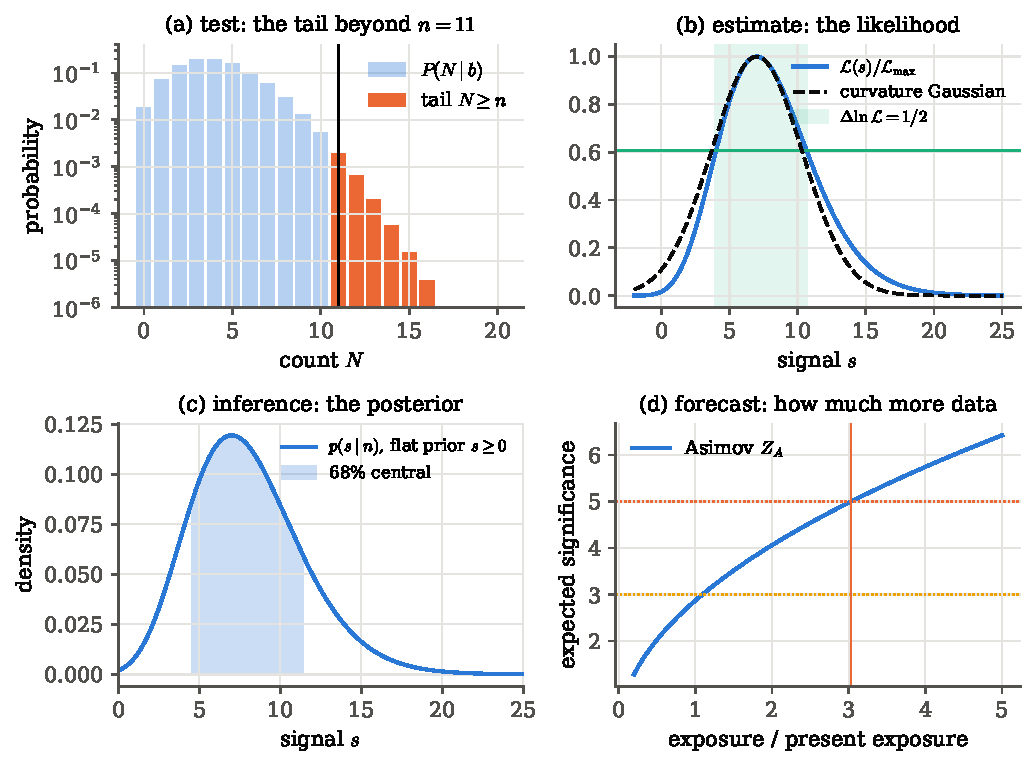
\includegraphics[width=0.95\linewidth]{figures/ch14/one_count.pdf}
\caption{One count, four objects. (a) The prediction of the background alone; the
orange bars are the outcomes at least as large as the eleven observed, and their total
is the p-value. (b) The same Poisson probability read as a function of the signal $s$;
the dashed Gaussian has the curvature at the peak, and the green band is where $\ln\Like$
is within $\frac12$ of its maximum. (c) The posterior for $s$ with a flat prior on
$s\ge0$, with its central $68\%$. (d) The expected significance as the exposure grows;
the vertical line marks the exposure that would give $5\sigma$.}
\label{14a:fig:one-count}
\end{figure}

\paragraph{What the example shows.}
None of the eight numbers is wrong, and none can replace another. The p-value of
$\ThOcPexact$ is not the probability that the background-only hypothesis is true; the
Bayes factor of $\ThOcBten$ depends on a prior range that the p-value never needed; the
curvature error $\pm\ThOcSigCurv$ is a Gaussian summary of a likelihood that is
lopsided; the forecast of $\ThOcKfive$ times the data assumes a signal that the data have
only hinted at. Every trap collected in \cref{14a:sec:pitfalls} is one of these objects
asked to answer a question that belongs to another.

\begin{keyidea}[the question first]
Say the question in words before computing anything. The question fixes the direction
(prediction or inference), and the direction fixes the object: a distribution, a
p-value, a likelihood, a posterior, an evidence or a forecast. A number is only as
meaningful as the match between the question asked and the object computed.
\end{keyidea}
\section{Which distribution, which method}\label{14a:sec:which}

Two choices come before any inference. The first is the distribution of the number
we measured: the machine that made it fixes how it scatters, and the scatter is the
likelihood. The second is the method that turns that distribution into an answer: a
forecast, a test, an interval, a posterior or a model comparison. Making the first
choice by fitting curves to a histogram, or the second by habit, is the commonest way
an analysis goes wrong without anyone noticing. Both choices can be made by asking a
few questions in a fixed order, and both orders can be drawn as decision charts.

\subsection{Which distribution: ask what made the number}\label{14a:sec:which-dist}

\Cref{2b:sec:which} gave the rule: the question ``which distribution?'' is really
``which machine made these numbers?'', and the histogram comes afterwards, to check
the answer in the tails, where the conclusion of a search rests. The machines met
since then add a few branches to the family trees drawn there: estimated spectra,
quadratic forms with simulated covariances, and summaries so elaborate that no
machine can be written down. \Cref{14a:fig:which-dist} arranges all of them as a
chart. Start at the left with the question \emph{how was the number made?}, follow
the branch that describes the operation, and read off the distribution.

\begin{figure}[htbp]
\centering
\begin{tikzpicture}[
  q/.style={draw=accent,thick,rounded corners=2pt,fill=ideabg,align=center,font=\footnotesize,
            text width=2.3cm,minimum height=0.9cm,inner sep=2pt},
  m/.style={draw=black!45,rounded corners=2pt,fill=white,align=left,font=\scriptsize,
            text width=3.5cm,minimum height=0.72cm,inner sep=2.5pt},
  d/.style={draw=formblue,rounded corners=2pt,fill=formblue!7,align=left,font=\scriptsize,
            text width=5.3cm,minimum height=0.72cm,inner sep=2.5pt},
  arr/.style={->,black!55}]
  \node[q] (root) at (0,0) {how was the\\ number made?};
  \foreach \y/\mm/\dd/\nm in {
     4.55/{counted events}/{fixed number of trials: binomial (a histogram with a fixed total: multinomial); constant rate, no memory: Poisson; fluctuating rate: negative binomial}/a,
     3.15/{summed or averaged many pieces}/{Gaussian (a vector of them: multivariate normal); pieces with no finite variance: Cauchy, Landau, no CLT}/b,
     1.95/{waited for events}/{first event: exponential; $k$-th event: gamma}/c,
     0.85/{multiplied positive factors}/{log-normal}/d,
     -0.35/{squared and added Gaussians}/{$\chi^2_\nu$; full-sky $\Chat$: $\Cell\chi^2_{2\ell+1}/(2\ell+1)$; masked sky: scaled $\chi^2_{\nu_{\rm eff}}$; several fields: Wishart}/e,
     -1.7/{took the length or power of a complex Gaussian}/{amplitude: Rayleigh; power: exponential ($\chi^2_2/2$); with a signal: noncentral}/f,
     -2.95/{divided by an estimated scale, or used a simulated covariance}/{Student $t$; $F$; Hotelling $T^2$ for $\bm r\T\hat\Cmat^{-1}\bm r$}/g,
     -4.25/{built an elaborate summary (peaks, Betti numbers, persistence)}/{no formula: simulate the summary through the same pipeline and histogram it}/h} {
    \node[m] (m\nm) at (3.6,\y) {\mm};
    \node[d] (d\nm) at (8.6,\y) {\dd};
    \draw[arr] (root.east) -- (m\nm.west);
    \draw[arr] (m\nm.east) -- (d\nm.west);
  }
\end{tikzpicture}
\caption{Which distribution, chosen by the operation that produced the number. The
middle column names the operation, the right column the distribution it produces, with
the variants that apply when the conditions change. The last row is where the book
ended up most often: summaries for which no machine can be written, whose distribution
is measured by simulation. Whatever the branch, the tails are checked separately,
because that is where tests and discoveries live.}
\label{14a:fig:which-dist}
\end{figure}

Three recognitions show the chart at work. Each one is a number the book met, read
off the chart and then checked with a short calculation.

\paragraph{Example: the matched filter with an unknown phase.}
A gravitational-wave search correlates the detector output with a template whose phase
is unknown, so it uses two templates a quarter cycle apart and combines their outputs
$z_c$ and $z_s$ (\cref{10b:sec:matched-filter}). In pure noise each output is a
standard normal, and the two are independent. \emph{How was the number made?} The
detection statistic $\rho^2=z_c^2+z_s^2$ is the power of a complex Gaussian, two squared
Gaussians added. The chart gives $\chi^2_2$, whose density is $\frac12e^{-x/2}$
(\cref{2b:sec:chi2}). The false-alarm probability above a threshold $x_*$ is then
\begin{align}
  \Prob(\rho^2>x_*\given\text{noise})
  &\eqby{1}\int_{x_*}^{\infty}\tfrac12e^{-x/2}\,\dd x
   \eqby{2}\Bigl[-e^{-x/2}\Bigr]_{x_*}^{\infty}
   \eqby{3}e^{-x_*/2}.
  \label{14a:eq:chi2-two}
\end{align}
\begin{explain}
  \item The tail of the $\chi^2_2$ density.
  \item The antiderivative of $\frac12e^{-x/2}$ is $-e^{-x/2}$.
  \item At the upper limit the exponential vanishes.
\end{explain}
A false-alarm probability of $10^{-3}$ per template therefore needs
$\rho_*=\sqrt{2\ln10^3}=3.72$, not the $3.09$ of a one-sided Gaussian: the unknown
phase is a second chance for the noise to look like a signal.

\paragraph{Example: a $\chi^2$ whose covariance came from simulations.}
In \cref{13b:sec:chi2} thirty-six Minkowski-functional values of the sky were combined
into one number $\bm r\T\hat\Cmat^{-1}\bm r$, with $\bm r$ the difference from the
simulated mean and $\hat\Cmat$ estimated from simulated skies. The chart sends this
number not to $\chi^2_{36}$ but to the branch ``used a simulated covariance''. Its mean
is $p(n-1)/(n-p-2)$ times too large for $p$ bins and $n$ simulations
(\cref{8b:sec:hartlap}), and even after that is corrected its tail is the
Hotelling law, a scaled $F$ distribution, rather than $\chi^2_p$
(\cref{12c:sec:hotelling}). \Cref{14a:sec:pitfall-cov} measures the size of the error.

\paragraph{Example: a bandpower on a cut sky.}
On the full sky the estimate $\Chat$ at one multipole is $\Cell\chi^2_{2\ell+1}/(2\ell+1)$
(\cref{7b:sec:chat}). With a mask the multipoles are mixed and no exact law is known,
but the chart's branch ``squared and added Gaussians'' still suggests a scaled
$\chi^2$, $X=\langle X\rangle\chi^2_\nu/\nu$, with the number of degrees of freedom
$\nu$ left free. It is fixed by matching the variance measured on simulations:
\begin{align}
  \Var X
  &\eqby{1}\frac{\langle X\rangle^2}{\nu^2}\Var\chi^2_\nu
   \eqby{2}\frac{\langle X\rangle^2}{\nu^2}\,2\nu
   \eqby{3}\frac{2\langle X\rangle^2}{\nu}
  \qquad\Longrightarrow\qquad
  \nu_{\rm eff}=\frac{2\langle X\rangle^2}{\Var X}.
  \label{14a:eq:nueff}
\end{align}
\begin{explain}
  \item A constant factor $c$ multiplies a variance by $c^2$, here $c=\langle X\rangle/\nu$.
  \item The variance of $\chi^2_\nu$ is $2\nu$ (\cref{2b:sec:chi2}).
  \item Cancel one factor of $\nu$, then solve for $\nu$.
\end{explain}
On the full sky this returns $\nu=2\ell+1$; on a cut sky $\nu_{\rm eff}$ comes out close
to $(2\ell+1)\fsky$ for smooth masks, and is measured, not assumed, for sharp ones
(\cref{8b:sec:distribution}). The machine fixes the family, and the simulations fix
the one number the machine could not.

\subsection{Which method: ask what is known and what is wanted}\label{14a:sec:which-method}

With the distribution of the summary in hand, the method follows from three questions
asked in order. \emph{Do we have data yet?} If not, the only question that makes sense
is how well a planned experiment could do, and the answer is a forecast. \emph{Is the
sampling distribution $P(S\given\params)$ known in closed form?} If not, it is built by
simulation before anything else. \emph{What do we want to know?} Whether the result
could be chance, which parameter values are allowed, which of two models is better,
or whether the model fits at all: four questions, four methods.
\Cref{14a:fig:which-method} draws the order.

\begin{figure}[htbp]
\centering
\begin{tikzpicture}[
  dec/.style={draw=accent,thick,diamond,aspect=2.4,fill=ideabg,align=center,font=\scriptsize,
              inner sep=0.5pt,text width=2.2cm},
  leaf/.style={draw=black!45,rounded corners=2pt,fill=white,align=left,font=\scriptsize,
               text width=6.4cm,inner sep=3pt,minimum height=0.8cm},
  arr/.style={->,black!60},
  tag/.style={font=\scriptsize\itshape,black!70}]
  \node[dec] (q1) at (0,0) {data yet?};
  \node[dec] (q2) at (0,-2.4) {$P(S\given\params)$ in closed form?};
  \node[dec] (q3) at (0,-6.5) {what is wanted?};
  \node[leaf] (f) at (6.6,0) {\textbf{no data: forecast.} Fisher matrix at a fiducial model (\cref{ch:10}); at low signal-to-noise or along degeneracies, a chain on noise-free mock data (\cref{10b:sec:validity})};
  \node[leaf] (s) at (6.6,-2.4) {\textbf{no formula: simulate first.} The sampling distribution through the same pipeline as the data (\cref{ch:06,ch:08,12c:sec:mc}); a Gaussian with simulated mean and covariance, Hartlap-corrected; or ABC (\cref{12c:sec:abc})};
  \node[leaf] (t) at (6.6,-4.5) {\textbf{chance?} A test: statistic, null distribution, p-value; the look-elsewhere correction if anything was scanned (\cref{ch:04}). Nothing seen: an upper limit with $\mathrm{CL}_s$ and its expected band (\cref{4b:sec:limits})};
  \node[leaf] (e) at (6.6,-6.1) {\textbf{which values?} Few parameters, near-Gaussian: curvature or profile likelihood, a grid (\cref{3b:sec:curvature,5b:sec:laplace}); many or curved: MCMC (\cref{ch:09}); systematics as nuisance parameters (\cref{4b:sec:templates})};
  \node[leaf] (c) at (6.6,-7.55) {\textbf{which model?} Evidence, Bayes factor, nested sampling, Savage--Dickey; if several survive, average them (\cref{ch:05})};
  \node[leaf] (g) at (6.6,-8.85) {\textbf{does it fit at all?} Goodness of fit, null tests, posterior predictive checks (\cref{4a:sec:gof})};
  \draw[arr] (q1) -- (f);
  \draw[arr] (q1) -- (q2);
  \draw[arr] (q2) -- (s);
  \draw[arr] (q2) -- (q3);
  \node[tag,anchor=east] at (-0.15,-1.2) {yes};
  \node[tag,anchor=east] at (-0.15,-4.45) {yes};
  \draw[arr] (s.south west) ++(0.3,0) -- ++(0,-0.2) -| (1.6,-5.4) -- (q3.north east);
  \draw[arr] (q3.east) -- ++(0.55,0) |- (t.west);
  \draw[arr] (q3.east) -- ++(0.55,0) |- (e.west);
  \draw[arr] (q3.east) -- ++(0.55,0) |- (c.west);
  \draw[arr] (q3.east) -- ++(0.55,0) |- (g.west);
\end{tikzpicture}
\caption{Which method, chosen by what is already known and what is wanted. A forecast
needs no data; a simulated sampling distribution rejoins the main line as soon as it
exists; the last decision splits by the question asked of the data, and each of the
four branches has its own object.}
\label{14a:fig:which-method}
\end{figure}

\paragraph{Estimation and comparison ask different questions.}
Two of the four branches look alike and are not. ``Which values?'' and ``which
model?'' can both be put to the question ``is the effect zero?''. The estimation
branch looks at the whole posterior of the effect and asks whether the values near
zero are among the credible ones. The comparison branch sets up a model in which the
effect is exactly zero and asks whether that model predicted the data better than a
model in which it is free. Kruschke's point is that both are legitimate and that they
pose the question at different levels, so they need not agree
\srcref{Kruschke}{\S12.3, pp.~352--354}. The comparison is meaningful only if an exactly
zero effect is physically plausible, and only if the alternative's prior is a real
statement about the effect \srcref{Kruschke}{\S12.4, p.~354}. In physics both
conditions often hold: a massless photon, $f_{\rm NL}=0$ from single-field inflation, a
dark-matter environment that either exists or does not. Where they do not hold, the
estimate is the more informative answer.

\paragraph{Example: a Bayes factor for the null with a wide posterior.}
A coin gives seven heads in fourteen tosses. Model $H_0$ says $\theta=\frac12$; model
$H_1$ says $\theta$ is uniform on $[0,1]$. The binomial coefficient $\binom{14}{7}$ is
common to both evidences and cancels, so
\begin{align}
  B_{01}
  &\eqby{1}\frac{(\tfrac12)^{14}}{\int_0^1\theta^7(1-\theta)^7\,\dd\theta}
   \eqby{2}\frac{2^{-14}}{7!\,7!/15!}
   \eqby{3}3.14 .
  \label{14a:eq:coin-bf}
\end{align}
\begin{explain}
  \item Each evidence is the probability of the observed sequence under the model,
        averaged over the model's prior (\cref{5c:sec:models}).
  \item The beta integral $\int_0^1\theta^{a-1}(1-\theta)^{b-1}\dd\theta=(a-1)!(b-1)!/(a+b-1)!$
        with $a=b=8$ (\cref{2b:sec:zoo}).
  \item $2^{-14}=6.10\times10^{-5}$ and $7!\,7!/15!=1.94\times10^{-5}$.
\end{explain}
The data favour ``exactly fair'' by about three to one, yet the posterior of $\theta$
under $H_1$ is a Beta$(8,8)$ whose $95\%$ highest-density interval runs from $0.27$ to
$0.73$ \srcref{Kruschke}{\S12.2.1.1, p.~347}. Both statements are true. The first
compares two predictions of the data. The second says how precisely $\theta$ is known,
and it is not known well at all. Reporting only the Bayes factor would suggest a
precision the data do not have. When several models survive a comparison, the
parameter posteriors can be averaged with the posterior model probabilities as
weights, so that no single model is pretended to be true (\cref{5c:sec:nested}).

\paragraph{Sampling distributions keep two jobs.}
Within the inference branches a Bayesian never uses the cloud of data sets that were
not observed. Kruschke stresses that this cloud is still the right tool for two
jobs \srcref{Kruschke}{\S11.5, pp.~329--330}: planning, where the experiment has not been
run and its possible outcomes are exactly what we want to know about, and checking,
where data simulated from the fitted model are compared with the real data to see
whether the model is any good. The forecast and ``does it fit?'' boxes of
\cref{14a:fig:which-method} are those two jobs.

\paragraph{Four walks through the chart.}
\emph{Can LISA see a dark-matter spike around an intermediate-mass black hole?} No
data exist, so the chart says forecast: the Fisher matrix of the waveform phase
(\cref{10b:sec:forecast}). The environment's effect is weak and nearly degenerate with
the chirp mass, which is exactly the situation in which the forecast must be checked
by a chain on noise-free mock data; at the signal-to-noise ratios LISA expects, the
chain's widths exceeded the Fisher widths by factors of up to two to four
(\cref{10b:sec:fisher-vs-mh}).
\emph{Is the topology of the \textit{Planck} temperature map that of a Gaussian
field?} The data exist; no formula gives the sampling distribution of Betti numbers on a
masked, beamed, noisy sphere, so the chart says simulate first; the question is
``could it be chance?'', so the method is a test with a simulated null and a p-value
counted from the simulations (\cref{13b:sec:question}).
\emph{What are the amplitude and tilt of the primordial spectrum?} The data exist;
the bandpowers are close to Gaussian with a simulated covariance, so the likelihood is
available once the covariance is simulated; the question is ``which values?'' with
two curved, correlated parameters, so the method is a Markov chain
(\cref{13a:sec:fit}).
\emph{Is there a new particle decaying to two photons near $125\,$GeV?} The data exist:
a histogram of the invariant mass of photon pairs (\cref{ch:T4}). Each bin is a
Poisson count, so the sampling distribution is known in closed form, but the shape of
the background is not predicted by theory: it is a smooth function fitted to the data,
and its coefficients are nuisance parameters (\cref{4b:sec:templates}). The question is
``could it be chance?'', so the method is a test with the profile likelihood ratio
$q_0$, whose distribution under the background alone is known asymptotically; because
the mass was scanned, the local p-value needs the look-elsewhere correction
(\cref{4b:sec:scan}). At masses where nothing is seen, the same likelihood answers the
other question, which signal strengths are excluded, with $\mathrm{CL}_s$ and the band of
limits the background alone would give (\cref{4b:sec:limits}). The search was run on
public ATLAS data in \cref{13d:sec:discovery,13d:sec:limits}.

\begin{keyidea}[two charts, two questions]
The distribution is fixed by the operation that made the number, not by the look of
its histogram. The method is fixed by three questions in order: are there data yet,
is the sampling distribution known in closed form, and what exactly do we want to
know.
\end{keyidea}
\section{The pipeline, and who built each arrow}\label{14a:sec:pipeline}

The very first chapter drew one chain, \eqref{0a:eq:workflow}: a physical model makes
a field or a data set; we choose which information in it matters; we compress the
data into a summary; we derive how the summary scatters for each value of the
parameters; and only then do we infer physics. At that point the chain was a promise.
Every later chapter built one or more of its arrows, and many arrows were built
twice, once where a formula exists and once where only simulation can do the job.
Seeing the finished chain with each chapter in its place answers a practical question:
faced with a new experiment, which parts of the book does each step need?

\begin{figure}[htbp]
\centering
\begin{tikzpicture}[
  st/.style={draw=accent,thick,rounded corners=2pt,fill=ideabg,align=center,font=\footnotesize,
             text width=3.6cm,minimum height=0.85cm},
  ch/.style={draw=black!30,rounded corners=1pt,fill=white,align=left,font=\scriptsize,
             text width=3.6cm,inner sep=2.5pt},
  flow/.style={->,thick,accent}]
  \node[st] (a) at (0,0)    {1.\ physical model};
  \node[st] (b) at (4.5,0)  {2.\ field or data set};
  \node[st] (c) at (9.0,0)  {3.\ choose what matters};
  \node[st] (d) at (9.0,-4.1) {4.\ construct a summary $S$};
  \node[st] (e) at (4.5,-4.1) {5.\ its sampling distribution $P(S\given\params)$};
  \node[st] (f) at (0,-4.1) {6.\ infer physics};
  \draw[flow] (a) -- (b); \draw[flow] (b) -- (c); \draw[flow] (c.east) -- ++(0.45,0) |- (d.east);
  \draw[flow] (d) -- (e); \draw[flow] (e) -- (f);
  \node[ch,anchor=north] at (0,-0.6) {\cref{ch:T1}: $\Lambda$CDM to $\Cell$, $P(k)$, $\kappa$\\ \cref{ch:T2}: chirps, environments, candles, tracers\\ \cref{ch:T3}: what shapes the sky has\\ \cref{ch:T4}: cross sections, mass peaks};
  \node[ch,anchor=north] at (4.5,-0.6) {\cref{ch:07}: one realisation of a field\\ \cref{ch:08}: beam, noise, mask\\ \cref{6b:sec:unfolding}: a detector's response\\ \cref{ch:11}: galaxies as a point sample\\ \cref{ch:13}: real maps and catalogues};
  \node[ch,anchor=north] at (9.0,-0.6) {\cref{ch:00}: the ladder of summaries\\ \cref{7a:sec:phases}: what $P(k)$ throws away\\ \cref{ch:12}: what survives a nuisance};
  \node[ch,anchor=north] at (9.0,-4.7) {\cref{ch:03}: estimators, sufficiency\\ \cref{ch:07,ch:08}: $\Chat$, pseudo-$\Cell$, MASTER\\ \cref{ch:11}: Landy--Szalay, FKP\\ \cref{ch:12}: Minkowski functionals, Betti numbers, persistence};
  \node[ch,anchor=north] at (4.5,-4.7) {\cref{ch:02}: distributions from machines\\ \cref{ch:03}: sampling distributions, bootstrap\\ \cref{ch:06}: Monte Carlo\\ \cref{ch:08}: simulated covariance, Hartlap\\ \cref{12c:sec:mc}: summaries as random numbers\\ \cref{4b:sec:templates}: histograms with nuisances};
  \node[ch,anchor=north] at (0,-4.7) {\cref{ch:04}: tests, intervals, look-elsewhere, $\mathrm{CL}_s$ limits\\ \cref{ch:05}: posteriors, evidence\\ \cref{ch:09}: MCMC\\ \cref{ch:10}: Fisher forecasts\\ \cref{ch:13}: the capstone fits};
\end{tikzpicture}
\caption{The pipeline of the book with the chapters that built each stage. The
probability rules of \cref{ch:01} are the language of every arrow, and the Python of
\cref{ch:T0} is the tool of every arrow; neither is listed.
The first three stages decide what is computed; the last three decide what it
means.}
\label{14a:fig:pipeline-chapters}
\end{figure}

\paragraph{Reading the chain from left to right.}
The first stage is physics, and in the book it was borrowed: the cosmological model
turns six numbers into the expected $\Cell$ and $P(k)$ (\cref{T1a:sec:machine}), and a
compact binary turns masses and an environment into a phase $\Psi(f)$
(\cref{T2a:sec:spa}), and a collision model turns a particle's mass and couplings into
a cross section, a number of expected events and a peak in the invariant mass
(\cref{ch:T4}). A model never predicts the data themselves, only their
statistics, because the data are one draw from a random process
(\cref{7a:sec:random-field}). The second stage is the instrument and the survey: what
the beam smooths, where the noise is added, which part of the sky is hidden, which
galaxies made it into the catalogue (\cref{8a:sec:model,13c:sec:weights}), and how a
particle detector smears and loses the energies it records. That last effect is
described by a response matrix measured on simulated events, and it can either be
folded into the prediction or, with care, undone in the data
(\cref{6b:sec:unfolding}). The third
stage is a decision rather than a calculation: which property of the field should
carry the physics. The power spectrum is the natural choice for a Gaussian field,
because it is then a sufficient summary (\cref{3b:sec:recipe}); for a field made
non-Gaussian by gravity, or for a question about robustness, shapes and topology
become candidates (\cref{12a:sec:nuisance}).

The fourth stage turns the decision into an estimator. The fifth is where the
probability of the book does most of its work: the sampling distribution
$P(S\given\params)$. For a few summaries it has a closed form, the $\chi^2_{2\ell+1}$ of a
full-sky $\Chat$, the Gaussian of a matched filter in Gaussian noise, or the product
of Poisson probabilities of a histogram of collision events. In the last case the
predicted signal and background shapes are themselves uncertain, and each uncertainty
enters as a nuisance parameter that is profiled or integrated away
(\cref{4b:sec:templates}). For most of the
summaries a research analysis actually uses, the masked pseudo-$\Cell$, the jackknifed
correlation function, the Betti numbers of a noisy map, it is measured by sending
simulated data through exactly the same code as the real data. The sixth stage reads
that distribution backwards. Tests and intervals do it in the frequentist way
(\cref{ch:04}), and a search that finds nothing turns the same test into an upper
limit on the signal, protected by the $\mathrm{CL}_s$ construction against excluding a
signal to which the experiment was not sensitive (\cref{4b:sec:limits}); posteriors in the Bayesian way (\cref{ch:05}), with chains when the
parameters are many (\cref{ch:09}); and forecasts do it before the data exist, by
replacing the data with their expected value (\cref{ch:10}).

\paragraph{Where formulas end and simulations begin.}
The same summary can be on either side of that line depending on what the instrument
did to the data. On the full sky the mean, the variance and the shape of $\Chat$ all
have formulas, and simulations only verify them. With a mask, the mean can still be
undone with a coupling matrix computed from the mask alone, but the covariance and the
shape are measured on simulations (\cref{8b:sec:distribution}). That is the line between
verification and research drawn in \cref{8a:sec:research}, and
\cref{14a:fig:formula-vs-sim} draws it for the summaries of the book.

\begin{figure}[htbp]
\centering
\begin{tikzpicture}[x=2.25cm,y=0.62cm,
  fo/.style={draw=formblue,fill=formblue!15,rounded corners=1pt,minimum width=1.9cm,
             minimum height=0.45cm,font=\scriptsize,execute at begin node={formula}},
  si/.style={draw=fibreorange,fill=fibreorange!18,rounded corners=1pt,minimum width=1.9cm,
             minimum height=0.45cm,font=\scriptsize,execute at begin node={simulated}},
  rl/.style={anchor=east,font=\scriptsize,align=right},
  cl/.style={font=\scriptsize\bfseries,align=center}]
  \node[cl] at (1,1) {mean}; \node[cl] at (2,1) {covariance}; \node[cl] at (3,1) {shape};
  \node[rl] at (0.45,0) {counts in a bin (Poisson)};
  \node[fo] at (1,0) {};
  \node[fo] at (2,0) {};
  \node[fo] at (3,0) {};
  \node[rl] at (0.45,-1) {full-sky $\Chat$};
  \node[fo] at (1,-1) {};
  \node[fo] at (2,-1) {};
  \node[fo] at (3,-1) {};
  \node[rl] at (0.45,-2) {matched filter in Gaussian noise};
  \node[fo] at (1,-2) {};
  \node[fo] at (2,-2) {};
  \node[fo] at (3,-2) {};
  \node[rl] at (0.45,-3) {masked pseudo-$\Cell$ (MASTER)};
  \node[fo] at (1,-3) {};
  \node[si] at (2,-3) {};
  \node[si] at (3,-3) {};
  \node[rl] at (0.45,-4) {galaxy $\hat\xi(s)$ with a survey window};
  \node[fo] at (1,-4) {};
  \node[si] at (2,-4) {};
  \node[si] at (3,-4) {};
  \node[rl] at (0.45,-5) {$\chi$ of a Gaussian field, no mask};
  \node[fo] at (1,-5) {};
  \node[si] at (2,-5) {};
  \node[si] at (3,-5) {};
  \node[rl] at (0.45,-6) {Betti numbers of a masked, noisy sky};
  \node[si] at (1,-6) {};
  \node[si] at (2,-6) {};
  \node[si] at (3,-6) {};
  \node[rl] at (0.45,-7) {peaks of a lognormal mass map};
  \node[si] at (1,-7) {};
  \node[si] at (2,-7) {};
  \node[si] at (3,-7) {};
\end{tikzpicture}
\caption{For each summary of the book, whether the mean, the covariance and the shape
of its sampling distribution came from a formula (blue) or had to be measured on
simulations (orange). Going down the list, the observation and the summary become
more realistic, and the simulations take over, first for the scatter and then for
everything.}
\label{14a:fig:formula-vs-sim}
\end{figure}

\paragraph{Example: the whole chain for one CMB amplitude.}
How precisely could a perfect CMB experiment measure the overall amplitude $A$ of the
temperature spectrum, $\Cell=A\,\Cell^{\rm fid}$? Follow the chain. The model gives
$\Cell^{\rm fid}$ (stage 1). The sky is one realisation, seen on a fraction $\fsky$ of
the sphere up to $\ell_{\max}$ without noise (stage 2). For a Gaussian sky the spectrum
holds everything (stage 3), estimated by $\Chat$ (stage 4), whose scatter is cosmic
variance (stage 5). The forecast of stage 6 is the CMB Fisher matrix of
\cref{10a:sec:cmb-derive}, here with one parameter and no noise:
\begin{align}
  F_{AA}
  &\eqby{1}\sum_{\ell=2}^{\ell_{\max}}\frac{(2\ell+1)\fsky}{2}
     \Bigl(\frac{\partial\Cell/\partial A}{\Cell}\Bigr)^2
   \eqby{2}\frac{\fsky}{2A^2}\sum_{\ell=2}^{\ell_{\max}}(2\ell+1)
   \eqby{3}\frac{\fsky\,[(\ell_{\max}+1)^2-4]}{2A^2}
   \equiv\frac{N_{\rm modes}}{2A^2},
  \label{14a:eq:amp-fisher}
\end{align}
\begin{explain}
  \item The CMB Fisher matrix with $N_\ell=0$, for the single parameter $A$.
  \item $\partial\Cell/\partial A=\Cell^{\rm fid}=\Cell/A$, so each term of the bracket is $1/A^2$.
  \item $\sum_{\ell=0}^{L}(2\ell+1)=(L+1)^2$, the number of $\alm$ up to $L$, minus the
        $1+3=4$ modes of $\ell=0,1$.
\end{explain}
so $\sigma_A/A=\sqrt{2/N_{\rm modes}}$: each independent mode measures the variance once,
and a variance measured from $N$ Gaussian numbers has a relative error $\sqrt{2/N}$
(\cref{3a:sec:var-of-var}). For $\ell_{\max}=2000$ and $\fsky=0.6$, $N_{\rm modes}=0.6\times(2001^2-4)
\approx2.4\times10^6$ and $\sigma_A/A\approx9\times10^{-4}$. \textit{Planck} measures
$\ln(10^{10}A_s)$ to $0.014$, an error of $1.4\%$ on $A_s$ \cite{Planck2018VI}, fifteen times
larger. The difference is not noise: the temperature spectrum measures only the
combination $A_se^{-2\tau}$, and the error on the optical depth $\tau$ is passed on to
$A_s$ (\cref{9c:sec:planck,T1a:sec:cl-response}). Stage 6 is where degeneracies between
parameters, not the count of modes, set the final error.

\paragraph{Example: the chain for a gravitational-wave amplitude.}
The detector records strain plus Gaussian noise with power spectral density $S_n(f)$
(stages 1 and 2, \cref{T2a:sec:lisa}). Because the noise is Gaussian and its
spectrum known, the data themselves are a sufficient summary and the likelihood is
exact: $\Like\propto e^{-(d-h|d-h)/2}$ with the noise-weighted inner product of
\cref{10b:sec:detection} (stages 3 to 5). For the overall amplitude, $h=\mathcal A\,g$
with $g$ fixed, the Fisher matrix of \cref{10b:sec:fisher} gives
\begin{align}
  \Gamma_{\ln\mathcal A\,\ln\mathcal A}
  &\eqby{1}\Bigl(\frac{\partial h}{\partial\ln\mathcal A}\Big|\frac{\partial h}{\partial\ln\mathcal A}\Bigr)
   \eqby{2}(h|h)
   \eqby{3}\rho^2,
  \qquad\sigma_{\ln\mathcal A}=\frac1\rho ,
  \label{14a:eq:gw-amp}
\end{align}
\begin{explain}
  \item The Gaussian-noise Fisher matrix, $\Gamma_{ij}=(\partial_ih|\partial_jh)$.
  \item $\partial h/\partial\ln\mathcal A=\mathcal A\,\partial h/\partial\mathcal A=\mathcal A g=h$.
  \item The squared signal-to-noise ratio is $\rho^2=(h|h)$.
\end{explain}
A source at $\rho=20$ has its amplitude measured to $5\%$, independent of everything
else about the waveform. Here the CMB example's lesson is reversed: the amplitude is
the easy parameter, and the hard ones are those whose effect on the phase other
parameters can imitate (\cref{10b:sec:fisher-structure}).

\paragraph{Example: the chain for the topology of the sky.}
The model is a Gaussian $\Lambda$CDM sky, possibly with a small $f_{\rm NL}$ (stage 1,
\cref{T3a:sec:nongauss}); the data are a masked, beamed, noisy temperature map (stage 2).
The choice of stage 3 is to look at the shape of the excursion sets at thresholds set
by the area fraction, which removes any monotone distortion of the temperature values
(\cref{12a:sec:mfs}). Stage 4 counts areas, boundary lengths, Euler characteristics and
Betti numbers inside the mask. For an unmasked Gaussian field the mean of the Euler
characteristic has a formula (\cref{12a:sec:gkf}); for everything else in stage 5 there
are only simulated skies sent through the same mask and code. Stage 6 is a test against
the Gaussian null with a simulated covariance (\cref{13b:sec:chi2}). The chain is the
same as for the amplitude; what moved is the line between formula and simulation in
\cref{14a:fig:formula-vs-sim}.

\paragraph{What the chain buys us.}
A new problem can be placed on the chain before any calculation. Its stage 5 decides
the cost: if the summary has a known sampling distribution, the analysis is a few
lines; if not, the number of simulations sets the precision of everything after it
(\cref{8b:sec:nsims}). Its stage 6 decides the dangers: the traps of
\cref{14a:sec:pitfalls} all live there.

\begin{inpractice}[the chain in a research collaboration]
A large analysis divides the chain among teams: a theory team owns the Boltzmann or
waveform code (stage 1), an instrument team the beam, noise and mask models and the
end-to-end simulations (stages 2 and 5), and an analysis team the estimators and the
likelihood (stages 4 and 6). The \textit{Planck} likelihood, the LIGO--Virgo parameter
estimation and the BOSS clustering analysis all have this shape. The weak points are
the hand-overs: a covariance simulated with a different mask from the one in the data,
or a template built at a different fiducial cosmology from the one used for the
distances, each passes silently from one stage to the next.
\end{inpractice}
\section{Four instruments, one likelihood}\label{14a:sec:universal}

A particle physicist scanning a diphoton spectrum, a cosmologist fitting the
\textit{Planck} temperature spectrum, a gravitational-wave astronomer estimating the
masses of a binary and a survey astronomer measuring the clustering of galaxies read
different journals and use different words. In \cref{0a:sec:universal} we saw that
underneath all of them lies one question: for a trial value of the parameters, how
probable is the noise realisation that would turn the model's prediction into the data
actually recorded? The likelihood is the density of that required noise
\eqref{0a:eq:like-noise}. At that point the claim rested on three short formulas. Now
every stage of the pipeline has been built for each instrument, and the comparison can
be made stage by stage. The interesting part is no longer that the idea is shared; it
is \emph{where} the four implementations differ, because each difference is a place
where a method that works for one instrument fails for another.

\begin{table}[htbp]
\centering
\footnotesize
\renewcommand{\arraystretch}{1.28}
\begin{tabularx}{\linewidth}{@{}>{\raggedright\arraybackslash}p{2.0cm}
  >{\raggedright\arraybackslash}X >{\raggedright\arraybackslash}X
  >{\raggedright\arraybackslash}X >{\raggedright\arraybackslash}X@{}}
\toprule
 & \textbf{collider counts} & \textbf{CMB} & \textbf{gravitational waves} & \textbf{LSS and topology}\\
\midrule
data & events in bins of mass & a temperature (and polarization) map & a strain time series & a galaxy catalogue, a mass map\\
noise & Poisson counting & cosmic variance of a Gaussian field, plus detector noise & stationary Gaussian noise with spectrum $S_n(f)$ & cosmic variance, shot noise, shape noise; non-Gaussian\\
summary & the counts themselves & $\Chat$, pseudo-$\Cell$ bandpowers & the data themselves, or the matched-filter output & $\hat\xi(s)$, $\hat P(k)$; peaks, Minkowski functionals, Betti numbers\\
its distribution & Poisson, exact & $\chi^2_{2\ell+1}$ (Wishart for several fields); simulated with a mask & Gaussian, exact & simulated (mocks, simulated maps)\\
$-2\ln\Like$ & $2\sum_i[\mu_i-n_i\ln\mu_i]$ & sum over $\ell$ of $(2\ell+1)\bigl[\Tr(\Cmat^{-1}\widehat{\Cmat})$ $+\ln\det\Cmat\bigr]$ & $(d-h\,|\,d-h)$ & $\bm r\T\hat\Cmat^{-1}\bm r$, $\bm r=\bm S-\hat{\bm\mu}$, Hartlap-corrected\\
$\params$ enters & the mean $\mu_i(\params)$, with nuisance parameters for the shapes & the covariance $\Cmat_\ell(\params)$ & the mean $h(\params)$ & mostly the mean; covariance fixed at a fiducial model\\
forecast & Asimov significance, $\sigma_s^2=(s+b)$ & Knox, CMB Fisher matrix & $\Gamma_{ij}=(\partial_ih|\partial_jh)$ & Fisher with simulated derivatives and its noise bias\\
many tests & the look-elsewhere effect in a mass scan & anomalies chosen after looking & a bank of templates and arrival times & many thresholds and summaries: combine, do not pick\\
built in & \cref{3b:sec:poisson,4a:sec:bump,4b:sec:scan,4b:sec:templates,4b:sec:limits,ch:T4,13d:sec:discovery,13d:sec:limits} & \cref{ch:07,ch:08,9c:sec:cl-like,ch:13} & \cref{ch:T2,10b:sec:detection,10b:sec:fisher} & \cref{ch:11,ch:12,12c:sec:mc}\\
\bottomrule
\end{tabularx}
\caption{The same pipeline in four instruments. Each column is one kind of experiment
and each row one stage of the analysis. The rows that differ, where the parameters
enter and whether the distribution is known or simulated, decide which methods
transfer from one column to another.}
\label{14a:tab:universal}
\end{table}

\paragraph{The question in words.}
For each instrument: what is the noise that the data require, what is its
distribution, and how do the parameters change it? The answers fill
\cref{14a:tab:universal}. Two of its rows deserve a derivation, because they are
where the columns part company: the form of the likelihood for counts and for a
Gaussian field with several components, and the place where the parameters enter.

\paragraph{Example: counts in many bins.}
A spectrum of $k$ independent bins with counts $n_i$ and expected counts
$\mu_i(\params)=s_i(\params)+b_i$ has the likelihood of \cref{3b:sec:poisson}:
\begin{align}
  -2\ln\Like(\params)
  &\eqby{1}-2\sum_{i=1}^{k}\ln\frac{\mu_i^{n_i}e^{-\mu_i}}{n_i!}
   \eqby{2}2\sum_{i=1}^{k}\bigl[\mu_i-n_i\ln\mu_i\bigr]+2\sum_{i=1}^{k}\ln n_i! \nonumber\\
  &\eqby{3}2\sum_{i=1}^{k}\bigl[\mu_i(\params)-n_i\ln\mu_i(\params)\bigr]+\text{const}.
  \label{14a:eq:cash}
\end{align}
\begin{explain}
  \item Independent bins multiply, so their logarithms add.
  \item $\ln(\mu^ne^{-\mu}/n!)=n\ln\mu-\mu-\ln n!$, multiplied by $-2$.
  \item The data's own term $\sum\ln n_i!$ does not depend on $\params$.
\end{explain}
This is Cash's statistic \cite{Cash1979}. The parameters enter only through the mean.
Nothing in it assumes many counts, which is why it, and not a $\chi^2$ with $\sqrt{n_i}$
errors, is right for the sparse tails where new particles are sought. Its price is
that the null distribution of the best bump, scanned over all masses, has no Wilks
theorem behind it (\cref{4b:sec:scan}). Panel (a) of \cref{14a:fig:four-instruments}
shows one background-only spectrum of $\ThFiNbins$ bins scanned bin by bin. Its largest
local excess, $Z=\ThFiZmax$, would be matched or beaten somewhere in $\ThFiPglob$ of all
background-only spectra; a $3\sigma$ local excess, with local probability
$\ThFiPthreeLoc$, appears somewhere in $\ThFiPthree$ of them.

\paragraph{Example: a CMB multipole with temperature and polarization.}
At one multipole $\ell$ the temperature and the $E$-mode polarization give, for each
$m$, a pair $\bm a_{\ell m}=(a^T_{\ell m},a^E_{\ell m})$. Isotropy makes different $m$
uncorrelated and gives every $m$ the same $2\times2$ covariance
\[
  \Cmat_\ell=\begin{pmatrix}C^{TT}_\ell & C^{TE}_\ell\\ C^{TE}_\ell & C^{EE}_\ell\end{pmatrix}
\]
(\cref{7b:sec:isotropy}). As in the one-field count of \cref{7b:sec:chat}, the
independent real numbers are the vector $\bm x_0=\bm a_{\ell0}$, which is real with
covariance $\Cmat_\ell$, and for each $m=1,\dots,\ell$ the real and imaginary parts
$\bm x_m$ and $\bm y_m$ of $\bm a_{\ell m}=\bm x_m+i\bm y_m$, each with covariance
$\Cmat_\ell/2$; the negative $m$ are fixed by the reality condition
$\bm a_{\ell,-m}=(-1)^m\bm a_{\ell m}^*$. \emph{What is the probability of the observed
$\bm a_{\ell m}$ if the spectra are $\Cmat_\ell$?} It is the product of the Gaussian
densities of these independent vectors, and each contributes
$\bm x\T\Sigma^{-1}\bm x+\ln\det\Sigma$ (plus a constant) to $-2\ln\Like$:
\begin{align}
  -2\ln\Like(\Cmat_\ell)
  &\eqby{1}\bm x_0\T\Cmat_\ell^{-1}\bm x_0+\ln\det\Cmat_\ell
     +\sum_{m=1}^{\ell}\Bigl[\bm x_m\T\bigl(\tfrac12\Cmat_\ell\bigr)^{-1}\bm x_m
     +\bm y_m\T\bigl(\tfrac12\Cmat_\ell\bigr)^{-1}\bm y_m+2\ln\det\bigl(\tfrac12\Cmat_\ell\bigr)\Bigr]+c_1
     \nonumber\\
  &\eqby{2}\bm x_0\T\Cmat_\ell^{-1}\bm x_0
     +2\sum_{m=1}^{\ell}\bigl[\bm x_m\T\Cmat_\ell^{-1}\bm x_m+\bm y_m\T\Cmat_\ell^{-1}\bm y_m\bigr]
     +(2\ell+1)\ln\det\Cmat_\ell+c_2
     \nonumber\\
  &\eqby{3}\sum_{m=-\ell}^{\ell}\bm a_{\ell m}^\dagger\Cmat_\ell^{-1}\bm a_{\ell m}
     +(2\ell+1)\ln\det\Cmat_\ell+c_2
     \nonumber\\
  &\eqby{4}\Tr\Bigl[\Cmat_\ell^{-1}\sum_{m=-\ell}^{\ell}\bm a_{\ell m}\bm a_{\ell m}^\dagger\Bigr]
     +(2\ell+1)\ln\det\Cmat_\ell+c_2
     \nonumber\\
  &\eqby{5}(2\ell+1)\Bigl[\Tr\bigl(\Cmat_\ell^{-1}\widehat{\Cmat}_\ell\bigr)+\ln\det\Cmat_\ell\Bigr]+c_2 .
  \label{14a:eq:wishart-like}
\end{align}
\begin{explain}
  \item The Gaussian density of each independent real vector; $c_1$ collects the
        factors of $2\pi$, which do not depend on $\Cmat_\ell$.
  \item $(\frac12\Cmat_\ell)^{-1}=2\Cmat_\ell^{-1}$, and for a $2\times2$ matrix
        $\det(\frac12\Cmat_\ell)=\frac14\det\Cmat_\ell$, so each $m\ge1$ gives
        $2\ln\det\Cmat_\ell$ plus a constant; with $m=0$ that is $1+2\ell$ copies of
        $\ln\det\Cmat_\ell$.
  \item For a real symmetric matrix $M$, $\bm a^\dagger M\bm a=\bm x\T M\bm x+\bm y\T M\bm y$:
        the cross terms $i\bm x\T M\bm y-i\bm y\T M\bm x$ cancel because
        $\bm x\T M\bm y=\bm y\T M\bm x$. By the reality condition $\bm a_{\ell,-m}$ gives
        the same value as $\bm a_{\ell m}$, so the factor $2$ is the sum over $\pm m$.
  \item A number is its own trace, and the trace is cyclic:
        $\bm a^\dagger M\bm a=\Tr(M\bm a\bm a^\dagger)$.
  \item Define the estimated spectrum matrix
        $\widehat{\Cmat}_\ell=\frac1{2\ell+1}\sum_m\bm a_{\ell m}\bm a_{\ell m}^\dagger$, the
        two-field version of $\Chat$; it is real because the $\pm m$ terms are complex
        conjugates.
\end{explain}
For one field, $\Tr(\Cmat^{-1}\widehat{\Cmat})+\ln\det\Cmat$ becomes $\Chat/\Cell+\ln\Cell$
and \eqref{14a:eq:wishart-like} is the exact full-sky likelihood of
\cref{9c:sec:cl-like}. Read the other way, as a distribution of the data
$(2\ell+1)\widehat{\Cmat}_\ell$ for fixed $\Cmat_\ell$, it is a Wishart distribution
with $2\ell+1$ degrees of freedom, the matrix version of $\chi^2_{2\ell+1}$ and the same
law that governs a covariance matrix estimated from simulations (\cref{8b:sec:hartlap}).
Here the parameters enter only through the \emph{covariance}, and at low $\ell$ the
likelihood is far from Gaussian in $\Cell$ (panel b of
\cref{14a:fig:four-instruments}): at $\ell=2$ there are only $\ThFiNuTwo$ modes, and
the likelihood has a long tail to large $\Cell$. Detector noise adds $\bm N_\ell$ to
$\Cmat_\ell$, and a mask replaces $2\ell+1$ by an effective number of modes close to
$(2\ell+1)\fsky$ (\cref{9c:sec:cl-like}).

\paragraph{Example: a gravitational-wave signal in Gaussian noise.}
For a detector with stationary Gaussian noise, the noise in different frequency bins is
independent, with variance set by $S_n(f)$, and the likelihood is
$\Like\propto\exp[-\frac12(d-h|d-h)]$ with the noise-weighted inner product
(\cref{10b:sec:detection}). The parameters enter only through the \emph{mean}, the
waveform $h(\params)$. When the phase is unknown the detection statistic is the
$\chi^2_2$ of \eqref{14a:eq:chi2-two} in noise and a noncentral $\chi^2_2$ with a
signal; at $\rho=\ThFiRho$ a threshold set for a false-alarm probability of $10^{-3}$
($\rho^2>\ThFiThr$) catches the signal with probability $\ThFiPdet$ (panel c).

\paragraph{Example: summaries with no formula.}
For a galaxy correlation function measured through a survey window, or for peak counts
and Betti numbers of a lognormal mass map, nothing is known in closed form. The
standard choice is a Gaussian likelihood whose mean $\hat{\bm\mu}(\params)$ and
covariance $\hat\Cmat$ are both measured on simulations, the covariance at one fiducial
model (\cref{11a:sec:research,12c:sec:mc}). The Gaussian form is an assumption, checked
by histogramming the simulated summaries, and the estimated covariance changes the
distribution of the $\chi^2$ even when the data are exactly Gaussian. Panel (d) shows
$\ThFiP$ summaries with a covariance from $\ThFiN$ simulations. After the Hartlap factor
the mean of the $\chi^2$ is right, $\ThFiMean$ against $\ThFiP$, but the tail is heavier:
the $5\%$ critical value of $\chi^2_{\ThFiP}$ is exceeded in $\ThFiFa$ of trials.

\begin{figure}[htbp]
\centering
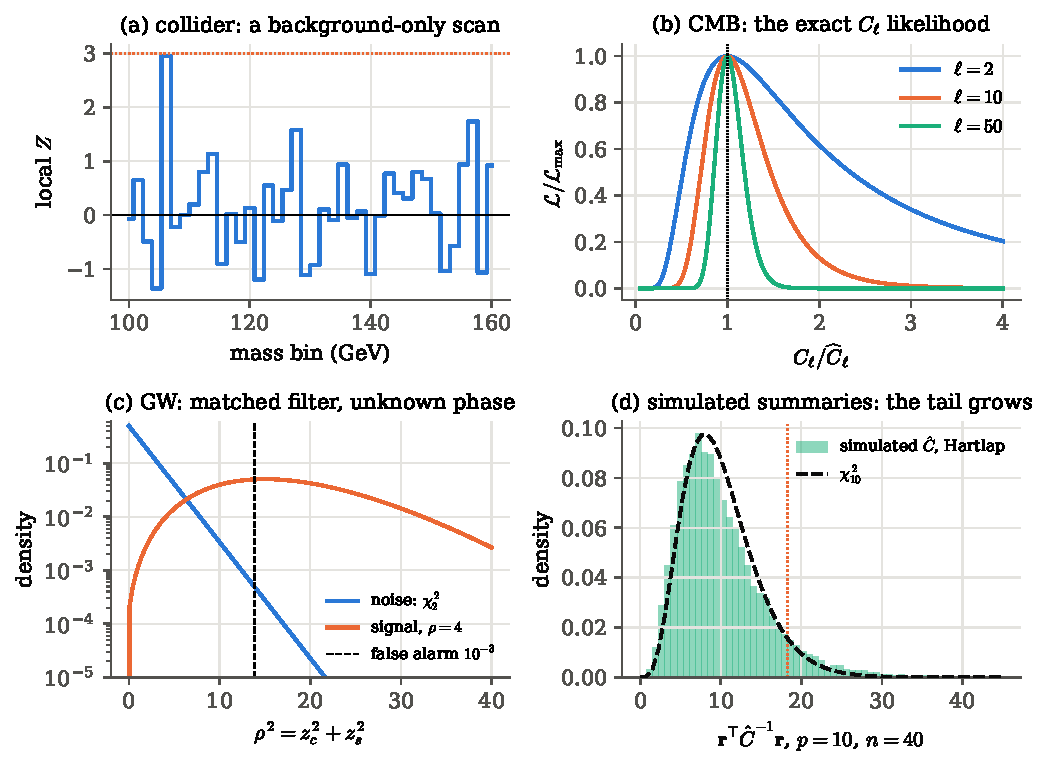
\includegraphics[width=0.95\linewidth]{figures/ch14/four_instruments.pdf}
\caption{The distribution each instrument's inference rests on. (a) A background-only
spectrum scanned bin by bin. When forty masses are tried, a local excess of two standard
deviations somewhere is common; the largest in this spectrum is $Z=\ThFiZmax$. (b) The exact likelihood of a CMB spectrum at one multipole,
when the measured $\Chat$ equals the fiducial value: lopsided at $\ell=2$, nearly
Gaussian at $\ell=50$. (c) The matched-filter statistic with an unknown phase, in noise
and with a signal of $\rho=4$; the dashed line is the threshold for a false-alarm
probability of $10^{-3}$. (d) A $\chi^2$ built with a covariance estimated from forty
simulations: after the Hartlap factor its mean is right but its tail is heavier than
$\chi^2_{10}$.}
\label{14a:fig:four-instruments}
\end{figure}

\paragraph{Where the parameters enter.}
All four likelihoods are, or are approximated by, a Gaussian in some data vector, with
\[
  -2\ln\Like(\params)=\bigl[\data-\bm\mu(\params)\bigr]\T\Cmat(\params)^{-1}\bigl[\data-\bm\mu(\params)\bigr]
  +\ln\det\Cmat(\params)+\text{const},
\]
the Poisson case joining through its Gaussian limit at large counts. The parameters can
sit in the mean, in the covariance, or in both, and the Fisher matrix inherits the
split: a mean part $\bm\mu_{,i}\T\Cmat^{-1}\bm\mu_{,j}$ and a covariance part
$\frac12\Tr[\Cmat^{-1}\Cmat_{,i}\Cmat^{-1}\Cmat_{,j}]$ (\cref{10a:sec:gauss}). The
consequences differ in practice. When the parameters sit in the mean, the likelihood is
Gaussian in the data even at low signal-to-noise, and the danger is a curved,
nonlinear model; this is the GW case, where the Fisher ellipse fails because the
waveform is not linear in its parameters (\cref{10b:sec:validity}). When they sit in
the covariance, the likelihood is not Gaussian in the data until many modes are
averaged; this is the CMB at low $\ell$, where a Gaussian approximation in $\Cell$
biases the answer (\cref{9c:sec:cl-like}). When neither is known, simulations supply
both, and their finite number becomes part of the error budget.
\Cref{14a:fig:where-theta} collects the three cases.

\begin{figure}[htbp]
\centering
\begin{tikzpicture}[
  top/.style={draw=accent,thick,rounded corners=2pt,fill=ideabg,align=center,font=\footnotesize,
              text width=8.6cm,inner sep=4pt},
  br/.style={draw=black!45,rounded corners=2pt,fill=white,align=left,font=\scriptsize,
             text width=3.9cm,inner sep=3pt,minimum height=2.6cm},
  arr/.style={->,thick,black!55}]
  \node[top] (t) at (4.5,0) {$-2\ln\Like=[\data-\bm\mu(\params)]\T\Cmat(\params)^{-1}[\data-\bm\mu(\params)]+\ln\det\Cmat(\params)$};
  \node[br,draw=formblue] (m) at (0,-2.6) {\textbf{$\params$ in the mean}\\[2pt]
     GW waveforms, a BAO template, a collider signal shape\\[2pt]
     Fisher: $\bm\mu_{,i}\T\Cmat^{-1}\bm\mu_{,j}$\\[2pt]
     breaks when $\bm\mu$ is curved in $\params$: low signal-to-noise, degeneracies};
  \node[br,draw=fibreorange] (c) at (4.5,-2.6) {\textbf{$\params$ in the covariance}\\[2pt]
     CMB $\Cell$, the $P(k)$ of a Gaussian field, cosmic shear\\[2pt]
     Fisher: $\tfrac12\Tr[\Cmat^{-1}\Cmat_{,i}\Cmat^{-1}\Cmat_{,j}]$\\[2pt]
     breaks when few modes are averaged: low $\ell$, large scales};
  \node[br,draw=tangentgreen] (s) at (9.0,-2.6) {\textbf{neither known: simulate}\\[2pt]
     masked spectra, $\hat\xi(s)$, peaks, Betti numbers\\[2pt]
     Fisher: simulated derivatives, minus their noise bias\\[2pt]
     breaks when simulations are too few: Hartlap, Hotelling};
  \draw[arr] (t.south) ++(-2.6,0) -- (m.north);
  \draw[arr] (t.south) -- (c.north);
  \draw[arr] (t.south) ++(2.6,0) -- (s.north);
\end{tikzpicture}
\caption{Where the parameters enter the likelihood decides how the analysis behaves. In
the mean (left), the likelihood stays Gaussian in the data and the trouble is a
nonlinear model. In the covariance (middle), the trouble is a non-Gaussian likelihood
when few modes are available. Measured from simulations (right), the trouble is the
finite number of simulations.}
\label{14a:fig:where-theta}
\end{figure}

\paragraph{Which methods transfer, and which do not.}
The table and the three cases explain why some recipes travel and others do not.
Inverting the Fisher matrix for a forecast transfers everywhere, but it is checked
against a chain in the left and right columns of \cref{14a:fig:where-theta} and
against the exact likelihood at low $\ell$ in the middle one. A $\chi^2$ with a known
covariance is exact for the gravitational-wave matched filter and for Gaussian
bandpowers at high $\ell$, approximate for counts, and has the Hotelling tail for
simulated summaries. The look-elsewhere correction is unavoidable in a mass scan, and
has analogues wherever many places, templates or thresholds are tried. The safest habit
for simulated summaries is to combine every threshold into one pre-declared statistic
rather than to quote the most significant one (\cref{12c:sec:test}).

\begin{keyidea}[same question, different noise]
The likelihood of every instrument is the probability of the noise that the data
require. What changes from one instrument to the next is where the parameters enter,
in the mean or in the covariance, and whether the distribution of the summary is known
or simulated. Those two facts decide which approximations hold and which checks are
needed.
\end{keyidea}
\section{The traps that kept coming back}\label{14a:sec:pitfalls}

The same few mistakes appeared in chapter after chapter, in coins, in collider bumps,
in CMB spectra and in gravitational waves. None of them is a mistake of arithmetic.
Each is a number built to answer one question being read as the answer to another,
exactly the mismatch the corridor example of \cref{14a:sec:questions} warned about.
Each trap has the same anatomy: the statement as people make it, the
everyday question it seems to answer, the assumption hidden inside that question, a
small simulated example that breaks the assumption (the numbers come from
\pyname{code/ch14/02_pitfalls.py}), and the lesson in one line.

\subsection{A p-value is not the probability that the null is true}\label{14a:sec:pitfall-p}

\emph{The statement.} ``We found $\pval=0.05$, so there is only a $5\%$ chance that
the effect is a fluke.''

\emph{The question it seems to answer.} Given what we saw, how probable is it that
nothing is there?

\emph{The hidden assumption.} The p-value runs in the forward direction: \emph{if} the
null were true, how often would a result this extreme or more appear
(\cref{4a:sec:pvalue-def})? The question runs backwards: given the result, how probable
is the null? Turning one into the other is Bayes' theorem, and Bayes' theorem needs two
things the p-value never used: how readily the \emph{alternative} would have produced the
same result, and how often nulls are true to begin with
(\cref{4a:sec:not-posterior}). The statement silently sets the first to one and ignores
the second.

\emph{An example where the assumption fails.} Picture a field in which half the
hypotheses tested are true nulls and the other half have real effects of varied size:
the true effect $\mu$, in units of the measurement error, is drawn from
$\Normal(0,\tau^2)$ with $\tau=\ThPaTau$, and each experiment reports
$z=\mu+\text{noise}$ with unit Gaussian noise and a two-sided p-value. Among the
experiments that landed near $p=0.05$, what fraction were true nulls? Under the null,
$z\sim\Normal(0,1)$. Under the alternative, $z$ is the sum of two independent Gaussians,
the effect and the noise, so it is Gaussian with the variances added,
$z\sim\Normal(0,1+\tau^2)$ (\cref{2b:sec:mvn}). The Bayes factor for the null at the
observed $z$ is the ratio of these two densities:
\begin{align}
  B_{01}
  &\eqby{1}\frac{e^{-z^2/2}/\sqrt{2\pi}}{e^{-z^2/2(1+\tau^2)}/\sqrt{2\pi(1+\tau^2)}}
   \eqby{2}\sqrt{1+\tau^2}\;\exp\Bigl[-\frac{z^2}{2}\Bigl(1-\frac{1}{1+\tau^2}\Bigr)\Bigr]
   \nonumber\\
  &\eqby{3}\sqrt{1+\tau^2}\;\exp\Bigl[-\frac{z^2}{2}\,\frac{\tau^2}{1+\tau^2}\Bigr]
   \eqby{4}\ThPaBzeroone .
  \label{14a:eq:b01-gauss}
\end{align}
\begin{explain}
  \item The two Gaussian densities at the observed $z$, variance $1$ under $H_0$ and
        $1+\tau^2$ under $H_1$.
  \item The $\sqrt{2\pi}$ cancels; the two exponentials combine into one.
  \item $1-1/(1+\tau^2)=\tau^2/(1+\tau^2)$.
  \item $z=1.96$ (the two-sided $p=0.05$) and $\tau=2$: $\sqrt5\,e^{-1.92\times0.8}$.
\end{explain}
With equal prior probabilities the posterior probability of the null is
$B_{01}/(1+B_{01})=\ThPaPostNull$. The simulation of $\ThPaN$ experiments agrees: of the
$\ThPaNsel$ that gave $0.045<p<0.055$, a fraction $\ThPaFracNull\pm\ThPaFracErr$ were
nulls (\cref{14a:fig:pitfalls-a}a). A different spread of effects gives a different
number, but there is a floor. Over every alternative that is symmetric about zero and
falls away from it, the most a p-value can support is the odds
$\bar B_{10}=-1/(e\,p\ln p)$ (\cref{5c:sec:pvalues}), which at $p=0.05$ is
$\ThPaBbar$, so the null keeps at least $\ThPaSellkePost$ of its probability.

\emph{The lesson.} A p-value is a prediction made from the null; the probability of the
null is an inference that needs the alternative and the prior, and at $p=0.05$ it is
nearer one third than one twentieth.

\begin{figure}[htbp]
\centering
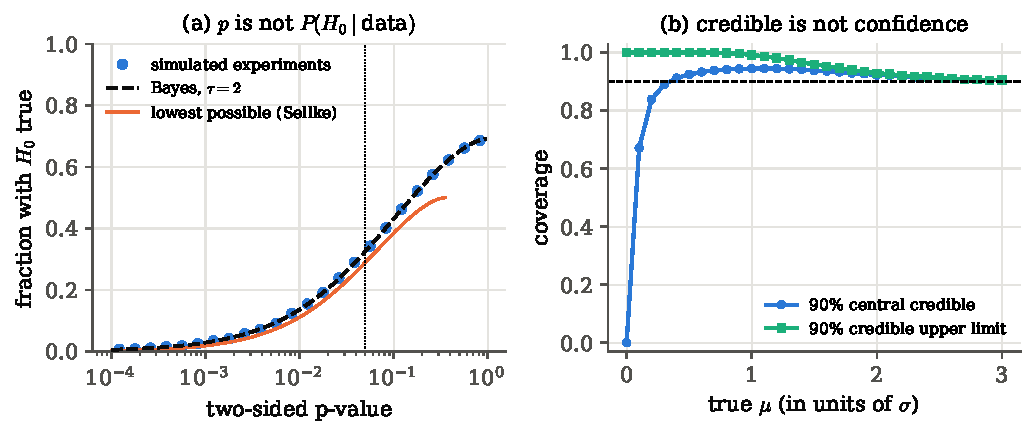
\includegraphics[width=0.95\linewidth]{figures/ch14/pitfalls_a.pdf}
\caption{(a) Among simulated experiments, half of them true nulls, the fraction of nulls
at each p-value. The dots are the simulation, the dashed curve the Bayes factor of
\eqref{14a:eq:b01-gauss}, and the orange curve the lowest value any symmetric,
decreasing alternative can produce. At $p=0.05$ (dotted line) about a third are nulls.
(b) How often a $90\%$ credible interval for a non-negative mean contains the truth, as
a function of the truth. The central interval never contains $\mu=0$; the upper limit
always does; neither has $90\%$ coverage near the boundary.}
\label{14a:fig:pitfalls-a}
\end{figure}

\subsection{A confidence interval is not a credible interval}\label{14a:sec:pitfall-ci}

\emph{The statement.} ``The $90\%$ interval is $[a,b]$, so the true value lies in
$[a,b]$ with probability $90\%$.''

\emph{The question it seems to answer.} How sure can we be that the parameter is in
this range, given the data we have?

\emph{The hidden assumption.} A confidence interval is a recipe whose output covers the
fixed true value in $90\%$ of repeated experiments (\cref{4b:sec:coverage}). The
probability belongs to the recipe, not to the one interval in hand. ``The value lies in
$[a,b]$ with probability $90\%$'' is a statement about the parameter given these data,
which is a credible interval and needs a prior (\cref{4b:sec:credible}). The two
coincide for a Gaussian mean far from any boundary with a flat prior, which is where
the habit is learned.

\emph{An example where the assumption fails.} A mass $\mu\ge0$ is measured once with
Gaussian error $\sigma=1$, and the reading is $x=\ThPbX$, below zero by a downward
fluctuation. The central $90\%$ confidence interval is $x\pm1.645=[\ThPbCIlo,\ThPbCIhi]$.
The recipe is valid: it covers the truth in $90\%$ of repetitions, whatever $\mu$ is. But
how much posterior probability does this particular interval hold? With a flat prior on
$\mu\ge0$ the posterior is the Gaussian $\Normal(x,1)$ cut at zero and renormalised, and
the interval's physical part is $[0,\ThPbCIhi]$:
\begin{align}
  \Prob(0\le\mu\le x+1.645\given x)
  &\eqby{1}\frac{\Phi(1.645)-\Phi(-x)}{1-\Phi(-x)}
   \eqby{2}\frac{0.950-0.933}{1-0.933}
   \eqby{3}\ThPbPostInCI .
  \label{14a:eq:ci-post}
\end{align}
\begin{explain}
  \item The probability of the Gaussian $\Normal(x,1)$ between $0$ and $x+1.645$, in units
        of standard deviations from $x$, divided by its total probability above zero.
  \item $-x=1.5$, and $\Phi(1.5)=0.933$.
  \item The script's value.
\end{explain}
So this ``$90\%$'' interval holds a quarter of the posterior probability. The reverse also
fails. The central $90\%$ credible interval, with $5\%$ of the posterior on each side,
never reaches down to zero, so if the true mass is zero it covers it in
$\ThPbCovZero$ of experiments; at $\mu=0.5$ it covers in $\ThPbCovHalf$, and only far from
the boundary, at $\mu=3$, does it settle at $\ThPbCovThree$. The credible upper limit
covers $\mu=0$ every time ($\ThPbCovUpZero$, \cref{14a:fig:pitfalls-a}b). A further
difference is what each depends on. For the same seven heads in twenty-four tosses,
Kruschke's one-tailed p-value, and with it the confidence interval, is $0.032$ if the
plan was to toss twenty-four times and $0.017$ if the plan was to stop at the seventh
head \srcref{Kruschke}{\S\S11.1.2--11.1.3, pp.~302--308}; the posterior is the same in
both cases, because the likelihoods are proportional (\cref{4a:sec:stopping}).

\emph{The lesson.} Coverage is a property of the recipe over repeated experiments,
credibility a property of the parameter given these data and a prior; check which one
the question asks for.

\subsection{A Fisher forecast is not the posterior}\label{14a:sec:pitfall-fisher}

\emph{The statement.} ``The Fisher matrix gives $\sigma=0.45$, so the experiment will
measure the parameter to $\pm0.45$.''

\emph{The question it seems to answer.} When the data come in, how wide will the
posterior be?

\emph{The hidden assumption.} The Fisher matrix is the average curvature of the
log-likelihood at the true parameters (\cref{10a:sec:fisher-def}). Its inverse is the
covariance of the posterior only if the log-likelihood is a quadratic in the
parameters, which is exact for a model linear in the parameters with Gaussian noise
and approximately true when the data are many (\cref{10a:sec:cr-reach}). Away from
that limit the posterior can be skewed, wider, or bounded, and the Gaussian of the
Fisher matrix cannot show it.

\emph{An example where the assumption fails.} $N$ unstable particles decay at times
$t_i$ drawn from $e^{-t/\tau}/\tau$, and we want the lifetime $\tau$. Write
$S=\sum_it_i$. The log-likelihood and the Fisher information are
\begin{align}
  \ln\Like(\tau)
  &\eqby{1}-N\ln\tau-\frac{S}{\tau},
  \qquad
  I(\tau)\eqby{2}-\E\Bigl[\frac{N}{\tau^2}-\frac{2S}{\tau^3}\Bigr]
         \eqby{3}-\frac{N}{\tau^2}+\frac{2N\tau}{\tau^3}
         \eqby{4}\frac{N}{\tau^2},
  \label{14a:eq:tau-fisher}
\end{align}
\begin{explain}
  \item The product of $N$ exponential densities, $\tau^{-N}e^{-S/\tau}$, in logarithms.
  \item The Fisher information is minus the expected second derivative; differentiate
        $-N\ln\tau-S/\tau$ twice.
  \item Each decay time has mean $\tau$, so $\E S=N\tau$.
  \item Collect the two terms.
\end{explain}
so the forecast is $\sigma_\tau=\tau/\sqrt N$. With a flat prior in $\tau$ the
posterior is the likelihood itself, $p(\tau\given S)\propto\tau^{-N}e^{-S/\tau}$. That
is the inverse-gamma shape $\tau^{-\alpha-1}e^{-\beta/\tau}$ with $\alpha=N-1$ and
$\beta=S$, whose mean is $\beta/(\alpha-1)=S/(N-2)$. Take the median experiment,
$S=N\tau$ with $\tau=1$. For $N=5$ the Fisher interval is
$[\ThPcFisherLoFive,\ThPcFisherHiFive]$; the posterior's central $68\%$ is
$[\ThPcLoFive,\ThPcHiFive]$, with median $\ThPcMedFive$ and mean $\ThPcMeanFive$. The
posterior is shifted up, more than twice as wide above the peak as below it, and
excludes the short lifetimes that the Fisher interval allows. For $N=50$ the two are
$[\ThPcFisherLoFifty,\ThPcFisherHiFifty]$ and $[\ThPcLoFifty,\ThPcHiFifty]$: the posterior
is approaching its Gaussian limit (\cref{14a:fig:pitfalls-b}a).

\emph{The lesson.} The Fisher matrix is the large-data limit of the posterior; whenever
the signal is weak, the model nonlinear or a parameter near a boundary, check the
forecast with a chain on mock data (\cref{10b:sec:validity}).

\begin{figure}[htbp]
\centering
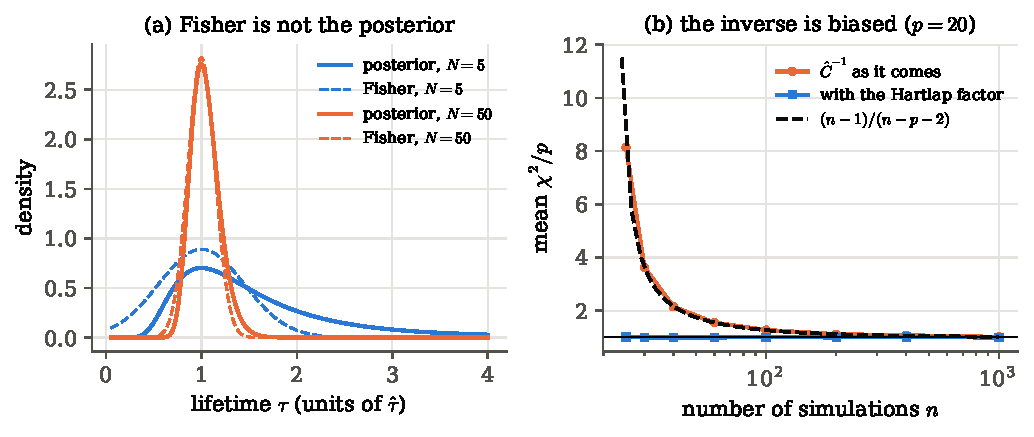
\includegraphics[width=0.95\linewidth]{figures/ch14/pitfalls_b.pdf}
\caption{(a) Posterior for a lifetime from $N=5$ and $N=50$ decays (solid), with the
Gaussian of the Fisher forecast (dashed), both for the median experiment. With five
decays the posterior is skewed towards long lifetimes and the forecast misplaces it;
with fifty the two nearly agree. (b) The mean of $\bm r\T\hat\Cmat^{-1}\bm r$ divided by
the number of bins $p=20$, for covariances estimated from $n$ simulations: the raw
inverse inflates it by $(n-1)/(n-p-2)$ (dashed), and the Hartlap factor removes the
inflation.}
\label{14a:fig:pitfalls-b}
\end{figure}

\subsection{A chain forgets where it started, not what it was told}\label{14a:sec:pitfall-start}

\emph{The statement.} ``We ran the chain long enough for the initial choices to wash
out.''

\emph{The question it seems to answer.} Does the answer still depend on anything we
chose before seeing the data?

\emph{The hidden assumption.} Two choices are made before the first step: the point
where the walker starts and the prior. Only the first is part of the walk. An ergodic
chain forgets its start geometrically fast (\cref{9a:sec:convergence}), but the prior is
part of the target density $\Like\times p$ that the chain samples
(\cref{9b:sec:start-prior}). A longer run only samples the posterior of that prior more
precisely.

\emph{An example where the assumption fails.} $N$ Gaussian readings of unit error have
mean $\bar x=1$, the true value. The prior, wrong and confident, is
$\Normal(\ThPdMuP,\ThPdSp^2)$. The posterior is Gaussian (\cref{5b:sec:conjugate}), with
mean
\begin{align}
  \E(\mu\given\data)
  &\eqby{1}\frac{\mu_p/s_p^2+N\bar x/\sigma^2}{1/s_p^2+N/\sigma^2}
   \eqby{2}\frac{-2/0.09+10}{1/0.09+10}
   \eqby{3}\ThPdTarget\quad(N=10),
  \label{14a:eq:wrong-prior}
\end{align}
\begin{explain}
  \item The inverse-variance weighted mean of the prior centre $\mu_p$ and the data mean
        $\bar x$ (the Normal--Normal update).
  \item $\mu_p=-2$, $s_p=0.3$, $\bar x=1$, $\sigma=1$, $N=10$.
  \item $-12.2/21.1$.
\end{explain}
Three Metropolis chains of $\ThPdNstep$ steps, started at $-20$, $0$ and $+20$, give
after a burn-in of $\ThPdBurn$ steps the means $\ThPdChainA$, $\ThPdChainB$ and
$\ThPdChainC$: the start is gone, and all three agree on the wrong answer
(\cref{14a:fig:pitfalls-c}a). More data do what more steps cannot. The data's weight
$N/\sigma^2$ grows while the prior's $1/s_p^2$ stays fixed, and the posterior mean moves
from $\ThPdPmOne$ at $N=1$ through $\ThPdPmHundred$ at $N=100$ to $\ThPdPmThousand$ at
$N=1000$ (\cref{14a:fig:pitfalls-c}b, and \cref{5b:sec:bvm}).

\emph{The lesson.} Steps remove the start, only data remove the prior; diagnose the
first with $\hat R$ and burn-in, and the second by rerunning with another prior.

\begin{figure}[htbp]
\centering
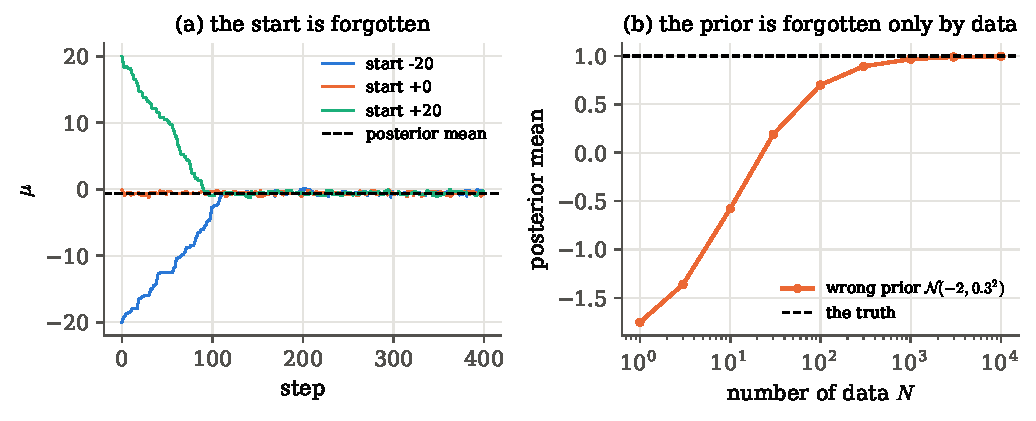
\includegraphics[width=0.95\linewidth]{figures/ch14/pitfalls_c.pdf}
\caption{(a) The first four hundred steps of three Metropolis chains started far apart,
for ten data points and a confident wrong prior: within about a hundred steps all three
wander around the same posterior mean (dashed), which is far from the truth $\mu=1$. (b)
The posterior mean with the same prior as the number of data grows: only data pull it
to the truth.}
\label{14a:fig:pitfalls-c}
\end{figure}

\subsection{The inverse of an estimated covariance is biased}\label{14a:sec:pitfall-cov}

\emph{The statement.} ``The sample covariance from simulations is unbiased, so its
inverse gives the right $\chi^2$.''

\emph{The question it seems to answer.} Is the scatter of my data vector properly
weighted?

\emph{The hidden assumption.} That the inverse of an unbiased estimate is an unbiased
estimate of the inverse. Inversion is a convex operation, so a fluctuation of a
variance towards zero raises its inverse more than an equal fluctuation away from zero
lowers it, and the average inverse is too large. For one bin and $n$ simulations the
factor is $(n-1)/(n-3)$ \eqref{8b:eq:inv-chi2}; for $p$ bins it is $(n-1)/(n-p-2)$
(\cref{8b:sec:hartlap}).

\emph{An example where the assumption fails.} Take $p=\ThPeP$ Gaussian summaries with
unit covariance, estimate the covariance from $n=30$ simulations, and compute the $\chi^2$
of an independent data vector, $\ThPeNtrial$ times. The mean should be $20$; it is
$\ThPeMeanThirty$, against the prediction $20\times29/8=\ThPeExpThirty$. At a nominal
$5\%$ threshold of $\chi^2_{20}$ the test rejects $\ThPeFaRawThirty$ of perfectly good data
sets. The Hartlap factor $(n-p-2)/(n-1)$ brings the mean to $\ThPeMeanHThirty$, but the
false-alarm rate is still $\ThPeFaHThirty$, because the tail of the corrected statistic
is the Hotelling law, not $\chi^2_p$ (\cref{12c:sec:hotelling}). With $n=100$ the raw
rate is $\ThPeFaRawHundred$ and the corrected one $\ThPeFaHHundred$
(\cref{14a:fig:pitfalls-b}b).

\emph{The lesson.} Correct the inverse, use the Hotelling (or a Student-type) likelihood
for the tail, and plan many more simulations than bins (\cref{8b:sec:nsims}).

\subsection{Where we looked changes how surprising it is}\label{14a:sec:pitfall-lee}

\emph{The statement.} ``A $3\sigma$ excess: a chance of one in seven hundred and forty.''

\emph{The question it seems to answer.} If there is nothing new, how often would we see
something this striking?

\emph{The hidden assumption.} That the excess was the only place we looked. If a bump
at any of $M$ masses would have been reported, the null distribution that answers the
question is that of the \emph{largest} excess among all $M$ (\cref{4b:sec:lee}).

\emph{An example where the assumption fails.} Let the $M$ search windows be independent,
each with local significance $Z_j\sim\Normal(0,1)$ under the background. The largest is
below a threshold $c$ only if every one of them is:
\begin{align}
  p_{\rm glob}
  &\eqby{1}1-\Prob\bigl(\max_jZ_j<c\bigr)
   \eqby{2}1-\prod_{j=1}^{M}\Prob(Z_j<c)
   \eqby{3}1-(1-p_{\rm loc})^M
   \relby{4}{\approx}Mp_{\rm loc}.
  \label{14a:eq:lee-indep}
\end{align}
\begin{explain}
  \item The complement of ``no window exceeds $c$''.
  \item Independent windows: the probability that all stay below $c$ is a product.
  \item Each factor is $1-p_{\rm loc}$ with $p_{\rm loc}=\Prob(Z>c)$.
  \item The binomial expansion to first order, valid while $Mp_{\rm loc}\ll1$.
\end{explain}
With $M=\ThPfM$ and $c=3$, $p_{\rm loc}=\ThPfPloc$ becomes $p_{\rm glob}=\ThPfPglob$
(simulated: $\ThPfPglobSim$), a global significance of $\ThPfZglob\sigma$ and a trials
factor of $\ThPfTrials$. Real windows overlap and are correlated, which lowers the
effective number of trials; the scan of \cref{4b:sec:scan} counted them with the
Gross--Vitells formula. Where the number of places looked at cannot be counted, as for
CMB anomalies noticed after the map was made (\cref{T3a:sec:planck}), no global p-value
can be computed at all.

\emph{The lesson.} The null distribution must describe the whole procedure, including
every place we would have been happy to find something.

\subsection{A shared calibration does not average down}\label{14a:sec:pitfall-cal}

\emph{The statement.} ``With a hundred independent measurements the error is ten times
smaller.''

\emph{The question it seems to answer.} How precise is the average?

\emph{The hidden assumption.} That the errors are independent. When every measurement
is multiplied or shifted by the same borrowed number, a zero point, the absolute
magnitude of a supernova, the sound horizon of a BAO analysis, that part of the error
is the same in all of them (\cref{11c:sec:h0-routes}).

\emph{An example where the assumption fails.} Each of $K$ measurements is
$x_i=\theta+c+e_i$, with independent errors $e_i$ of size $\sigma$ and a common offset
$c$ of size $\sigma_c$. The average is $\bar x=\theta+c+\frac1K\sum_ie_i$, so
\begin{align}
  \Var\bar x
  &\eqby{1}\Var c+\Var\Bigl(\frac1K\sum_{i=1}^Ke_i\Bigr)
   \eqby{2}\sigma_c^2+\frac{\sigma^2}{K}.
  \label{14a:eq:calib}
\end{align}
\begin{explain}
  \item The offset and the individual errors are independent, so their variances add.
  \item The variance of a mean of $K$ independent errors is $\sigma^2/K$
        (\cref{3a:sec:var-mean}).
\end{explain}
With $\sigma=\ThPgStat\%$ and $\sigma_c=\ThPgCal\%$, one measurement has an error of
$\ThPgTotOne\%$ and a hundred have $\ThPgTotHundred\%$ (simulated: $\ThPgSimHundred\%$),
not $0.2\%$. For the Hubble constant from supernovae, an offset $\delta M$ in the absolute
magnitude moves every distance together, $\delta H_0/H_0=(\ln10/5)\,\delta M$, and the
whole Hubble tension is an offset of $0.18$\,mag, about $8\%$ in $H_0$
(\cref{3b:sec:hubble,11c:sec:h0-routes}).

\emph{The lesson.} Find the factor that every measurement shares before averaging; its
error is a floor that no amount of data removes.

\paragraph{What the machinery assumes.}
The seven traps are special cases of a short list of assumptions that run through the
whole book. Each holds in the examples where a method was first derived, and each
fails somewhere in research. The table names the assumption, the place it breaks, and
what the data show when it does.

\begin{taxonomy}[assumptions, where they break, and the symptom]
\footnotesize
\renewcommand{\arraystretch}{1.25}
\begin{tabularx}{\linewidth}{@{}>{\raggedright\arraybackslash}p{3.5cm}
  >{\raggedright\arraybackslash}X >{\raggedright\arraybackslash}X@{}}
\toprule
\textbf{assumption} & \textbf{where it breaks} & \textbf{symptom, and the check}\\
\midrule
the likelihood is Gaussian in the parameters & few counts, low $\ell$, weak signals, nonlinear models & skewed chains; Fisher errors too small (\cref{10b:sec:validity,9c:sec:cl-like})\\
the data points are independent & a shared calibration, correlated bins, overlapping windows & errors that stop shrinking; $\chi^2$ per degree of freedom far from one (\cref{3a:sec:weighted})\\
the covariance is known & covariances from simulations or jackknife & inflated $\chi^2$, too many rejections (\cref{8b:sec:hartlap,13c:sec:jk-bias})\\
one test was made & mass scans, many thresholds, anomalies found by looking & excesses that fade with more data (\cref{4b:sec:lee})\\
the chain has converged & multiple modes, long correlation times & $\hat R>1$, different answers from different starts (\cref{9b:sec:rhat})\\
the prior is harmless & few data, wide prior ranges in model comparison & answers that move when the prior moves (\cref{5b:sec:bvm,5c:sec:prior-width})\\
the sample is the population & flux limits, survey masks, fibre collisions & biased distances and clustering (\cref{T2b:sec:malmquist,13c:sec:weights})\\
the model is right & any real data & poor goodness of fit; posterior predictive checks fail (\cref{4a:sec:gof})\\
\bottomrule
\end{tabularx}
\end{taxonomy}
\section{The words, and the routes through them}\label{14a:sec:glossary}

Statistics reuses ordinary words for precise things, and two words that sound alike
can belong to opposite directions of reasoning. ``Likely'' and ``probable'',
``error'' and ``uncertainty'', ``confidence'' and ``credibility'' are interchangeable in
conversation and not interchangeable in a paper. Every trap measured in
\cref{14a:sec:pitfalls} began with one of these swaps. Pinning each word to a plain
sentence and to the place where it was built removes the ambiguity. The words fall
into the groups the pipeline of \cref{14a:sec:pipeline} uses: the language of
probability, the estimate and its likelihood, tests and intervals, the Bayesian
objects, simulation and chains, and the fields, forecasts and summaries of research
analyses.

One word needs its two meanings stated before any table, because the others inherit
them. A \newterm{probability} can be a long-run frequency: the fraction of repeated
experiments in which something happens. That is the only reading the frequentist
school allows, and with it a parameter, being a fixed constant, has no probability at
all \mainref{p.~175}. Or it can be a degree of belief: how strongly the information we
hold supports a statement, including a statement about a constant such as the
electron mass \srcref{Cowan}{\S1.2, pp.~5--6}. Both obey the same rules of
\cref{1a:sec:axioms}. The forward objects of \cref{14a:fig:directions} can be read
either way; the backward ones need the second reading. In large samples with a
well-behaved model the two schools give nearly the same numbers, and in general they
need not \mainref{p.~185}, which is why every entry below says which question its
object answers.

\begin{center}
\small
\renewcommand{\arraystretch}{1.18}
\begin{tabularx}{\linewidth}{@{}>{\raggedright\arraybackslash}p{3.0cm}
                               >{\raggedright\arraybackslash}X
                               >{\raggedright\arraybackslash}p{2.0cm}@{}}
\toprule
\multicolumn{3}{@{}l}{\textbf{The language of probability}}\\
word & what it means here & built in\\\midrule
conditional probability & the probability after keeping only the cases in which $B$ happened, $\Prob(A\given B)=\Prob(A\cap B)/\Prob(B)$ & \cref{1a:sec:conditional}\\
independence & knowing that $B$ happened does not change the probability of $A$ & \cref{1a:sec:independence}\\
random variable & a number attached to each outcome of an experiment & \cref{1b:sec:rv}\\
pmf, pdf & probability of each value of a count; probability per unit length of a continuous number & \cref{1b:sec:pdf}\\
marginal distribution & the distribution of one variable with the nuisance variables averaged out of the joint distribution & \cref{1b:sec:marginal}\\
expectation, variance & the probability-weighted average; the average squared distance from it & \cref{1b:sec:expectation}\\
covariance, correlation & how two numbers move together; the same scaled to lie between $-1$ and $1$ & \cref{1b:sec:covariance}\\
Bernoulli, binomial & a single yes--no trial; the number of successes in many successive trials & \cref{2a:sec:bernoulli,2a:sec:binomial}\\
Poisson & the count of rare, independent events at a constant rate in a fixed window & \cref{2a:sec:poisson-inputs}\\
central limit theorem & a sum of many independent pieces with finite variance is close to Gaussian & \cref{2b:sec:clt}\\
$\chi^2_\nu$ & the sum of $\nu$ squared independent standard Gaussians & \cref{2b:sec:chi2}\\
multivariate normal & Gaussian numbers with a covariance matrix; every marginal and conditional is again Gaussian & \cref{2b:sec:mvn}\\
\bottomrule
\end{tabularx}
\end{center}

\begin{center}
\small
\renewcommand{\arraystretch}{1.18}
\begin{tabularx}{\linewidth}{@{}>{\raggedright\arraybackslash}p{3.0cm}
                               >{\raggedright\arraybackslash}X
                               >{\raggedright\arraybackslash}p{2.0cm}@{}}
\toprule
\multicolumn{3}{@{}l}{\textbf{The estimate and its likelihood}}\\
word & what it means here & built in\\\midrule
estimator & a recipe that turns data into a guess of a parameter; itself a random number & \cref{3a:sec:estimator}\\
sampling distribution & how the estimator scatters over repeated experiments at a fixed true value & \cref{3a:sec:sampdist}\\
bias, MSE & the average offset of the estimator from the truth; bias squared plus variance & \cref{3a:sec:mse}\\
standard deviation, standard error & the scatter of one measurement; the scatter of their mean, smaller by $\sqrt N$ & \cref{3a:sec:var-mean}\\
likelihood & for a trial $\params$, the probability of the noise needed to turn the prediction into the data seen; a function of $\params$, not a density in $\params$ & \cref{3b:sec:likelihood,3b:sec:not-density}\\
maximum-likelihood estimate & the $\params$ under which the observed data were most probable & \cref{3b:sec:mle}\\
Fisher information & the expected curvature of $-\ln\Like$; large curvature means a sharp estimate & \cref{3b:sec:fisher-info}\\
Cram\'er--Rao bound & no unbiased estimator scatters less than the inverse Fisher information & \cref{3b:sec:cramer-rao}\\
nuisance parameter & a parameter we must model but do not want, removed by profiling or integrating & \cref{3b:sec:profile,4b:sec:nuisance-hep}\\
profile likelihood & the likelihood of the wanted parameter with the nuisance parameters at their best value for it & \cref{3b:sec:profile}\\
sufficient statistic & a summary that keeps every piece of information the data carry about $\params$ & \cref{3b:sec:recipe-suff}\\
least squares & maximum likelihood when the noise is Gaussian with known widths & \cref{3b:sec:ls-from-ml}\\
bootstrap & the sampling distribution estimated by resampling the data themselves & \cref{3b:sec:bootstrap}\\
\bottomrule
\end{tabularx}
\end{center}

\begin{center}
\small
\renewcommand{\arraystretch}{1.18}
\begin{tabularx}{\linewidth}{@{}>{\raggedright\arraybackslash}p{3.0cm}
                               >{\raggedright\arraybackslash}X
                               >{\raggedright\arraybackslash}p{2.0cm}@{}}
\toprule
\multicolumn{3}{@{}l}{\textbf{Tests and intervals}}\\
word & what it means here & built in\\\midrule
null hypothesis & the hypothesis whose sampling distribution we know, usually ``it happened by chance'' & \cref{4a:sec:null}\\
p-value & if the null were true, the probability of a result like this one or further in the same direction & \cref{4a:sec:pvalue-def}\\
significance $Z$ & the p-value restated as the number of Gaussian standard deviations with the same one-sided tail & \cref{4a:sec:p-to-z}\\
size, power & the rate of false alarms we accept; the probability of detecting a real effect of given size & \cref{4a:sec:errors,4a:sec:power}\\
likelihood ratio, Wilks & best fit under the null over best fit overall; $-2\ln$ of it is $\chi^2$ for large samples & \cref{4a:sec:lrt,4a:sec:wilks}\\
confidence interval & a procedure whose intervals contain the true value in a stated fraction of repetitions & \cref{4b:sec:ci-def}\\
coverage & that fraction, measured by simulation at each true value & \cref{4b:sec:coverage}\\
Feldman--Cousins & a confidence belt ordered by likelihood ratio, which moves smoothly from limits to two-sided intervals & \cref{4b:sec:fc}\\
look-elsewhere effect & the extra chance of a large fluctuation somewhere when many places were searched & \cref{4b:sec:lee}\\
$\mathrm{CL}_s$ & the p-value of signal plus background divided by that of background alone; excludes only signals the experiment could see & \cref{4b:sec:cls-hep}\\
Asimov data, Brazil band & the data replaced by their expected values; the band of limits expected from background alone & \cref{4b:sec:asimov,4b:sec:brazil}\\
goodness of fit & whether the best model is an acceptable description at all & \cref{4a:sec:gof}\\
\bottomrule
\end{tabularx}
\end{center}

\begin{center}
\small
\renewcommand{\arraystretch}{1.18}
\begin{tabularx}{\linewidth}{@{}>{\raggedright\arraybackslash}p{3.0cm}
                               >{\raggedright\arraybackslash}X
                               >{\raggedright\arraybackslash}p{2.0cm}@{}}
\toprule
\multicolumn{3}{@{}l}{\textbf{The Bayesian objects}}\\
word & what it means here & built in\\\midrule
prior & how probable each parameter value was before these data & \cref{5b:sec:priors}\\
posterior & the prior reweighted by how readily each value could have produced the data, then normalised & \cref{5b:sec:continuous}\\
conjugate prior & a prior whose posterior has the same family, so the update is a change of two numbers & \cref{5b:sec:conjugate}\\
credible interval, HDI & a region holding a stated posterior probability; the narrowest such region & \cref{4b:sec:credible-def,4b:sec:hdi}\\
Bernstein--von Mises & with enough data the posterior forgets a smooth prior and becomes the Gaussian of the likelihood & \cref{5b:sec:bvm}\\
evidence & the probability a model gave to the data actually seen, averaged over its prior & \cref{5c:sec:evidence}\\
Bayes factor & the ratio of two evidences: which model predicted the data better & \cref{5c:sec:bf}\\
Occam factor & the fraction of a model's prior range that the data allow; the price of flexibility & \cref{5c:sec:occam}\\
Savage--Dickey ratio & for nested models, posterior over prior density at the null value & \cref{5c:sec:sddr}\\
model averaging & posteriors of several models combined with their posterior probabilities as weights & \cref{5c:sec:averaging}\\
\bottomrule
\end{tabularx}
\end{center}

\begin{center}
\small
\renewcommand{\arraystretch}{1.18}
\begin{tabularx}{\linewidth}{@{}>{\raggedright\arraybackslash}p{3.0cm}
                               >{\raggedright\arraybackslash}X
                               >{\raggedright\arraybackslash}p{2.0cm}@{}}
\toprule
\multicolumn{3}{@{}l}{\textbf{Simulation and chains}}\\
word & what it means here & built in\\\midrule
pseudo-random numbers, seed & a deterministic sequence that passes tests of randomness; the number that fixes it & \cref{6a:sec:seeds}\\
Monte Carlo error & the scatter of a simulated average, falling as $1/\sqrt N$ & \cref{6b:sec:sqrtN}\\
importance sampling & drawing from a convenient density and reweighting, with thicker tails than the target & \cref{6b:sec:importance}\\
response matrix, unfolding & the probability that a true bin lands in each measured bin, learned by simulation; its regularised inversion & \cref{6b:sec:unfolding}\\
stationary distribution & the distribution a Markov chain keeps once it has reached it & \cref{9a:sec:stationary}\\
detailed balance & equal probability flow each way between any two states; enough for stationarity & \cref{9a:sec:detailed-balance}\\
Metropolis--Hastings & a random walk biased by an accept--reject step to spend more time where the probability is higher & \cref{9b:sec:hastings}\\
burn-in & the early steps that still remember the starting point & \cref{9b:sec:burnin}\\
autocorrelation time & how many steps the chain needs to produce one independent draw & \cref{9b:sec:tau}\\
$\hat R$ & chains from different starts compared; values above one mean they have not met & \cref{9b:sec:rhat}\\
\bottomrule
\end{tabularx}
\end{center}

\begin{center}
\small
\renewcommand{\arraystretch}{1.18}
\begin{tabularx}{\linewidth}{@{}>{\raggedright\arraybackslash}p{3.0cm}
                               >{\raggedright\arraybackslash}X
                               >{\raggedright\arraybackslash}p{2.0cm}@{}}
\toprule
\multicolumn{3}{@{}l}{\textbf{Fields, forecasts and summaries}}\\
word & what it means here & built in\\\midrule
random field & a field whose values are random, described by their joint distribution at all points & \cref{7a:sec:random-field}\\
homogeneity, isotropy & the statistics do not change from place to place, or with direction & \cref{7a:sec:homog}\\
$\Cell$, $\Chat$ & the variance of the harmonic coefficients at multipole $\ell$; its estimate from one sky & \cref{7b:sec:chat}\\
cosmic variance & the scatter of $\Chat$ because only $2\ell+1$ modes exist at each $\ell$ & \cref{7b:sec:cosmic-variance}\\
pseudo-$\Cell$, MASTER & the spectrum of a masked sky; its mean undone with a mode-coupling matrix & \cref{8b:sec:pseudo,8b:sec:master}\\
Hartlap factor & the correction for the bias of the inverse of a covariance estimated from simulations & \cref{8b:sec:hartlap}\\
jackknife & a covariance from the data by leaving out one region at a time & \cref{13c:sec:jackknife}\\
Fisher forecast & the curvature of the expected log-likelihood at a fiducial model, before any data & \cref{10a:sec:fisher-def}\\
noise spectrum, matched filter & the variance of the noise per frequency; the correlation of the data with a template, weighted by it & \cref{10b:sec:psd,10b:sec:matched-filter}\\
excursion set, Minkowski functionals & the region above a threshold; its area, boundary length and Euler characteristic & \cref{12a:sec:excursion,12a:sec:mfs}\\
Betti numbers, persistence & the numbers of pieces and holes; the thresholds at which each is born and dies & \cref{T3a:sec:betti,12b:sec:filtration}\\
ABC & inference that keeps the parameter draws whose simulated summary lands near the observed one & \cref{12c:sec:abc}\\
\bottomrule
\end{tabularx}
\end{center}

\paragraph{Routes through the book.}
A glossary answers ``what does this word mean?''. A new analysis asks a different
question: which chapters does it need, and in what order? The pipeline of
\cref{14a:fig:pipeline-chapters} answers by stage. A shorter answer comes from
following the four instruments of \cref{14a:sec:universal} through the book, one
route each (\cref{14a:fig:routes}). The routes share their first stops, the rules of
probability and the distributions that come from machines, and part ways at the stage
where the instrument decides what the noise is. Each route starts from the Python of
\cref{ch:T0}, which every chapter uses. Its section on numerical trust (\cref{T0a:sec:trust}) asks a question that every
number in this book had to answer before it was printed: is the result a property of
the data, or of the rounding, the step size and the random seed that produced it?

\begin{figure}[htbp]
\centering
\begin{tikzpicture}[
  stop/.style={draw=black!45,rounded corners=2pt,fill=white,align=center,font=\scriptsize,
               text width=1.3cm,minimum height=1.0cm,inner sep=1.5pt},
  goal/.style={font=\footnotesize\bfseries,anchor=south west,inner sep=1pt},
  link/.style={->,thick}]
  \providecommand*{\fourteenaRoute}[5]{%
    \node[goal,text=#2] at (-0.7,#3+0.62) {#4};
    \foreach \i/\t in {#5} {\node[stop,draw=#2] (#1\i) at (1.78*\i,#3) {\t};}
  }
  \fourteenaRoute{a}{bdryred}{0}{a search for a new particle in counts}
    {0/{\ref{ch:02}\\ Poisson},1/{\ref{ch:03}\\ profile likelihood},2/{\ref{ch:04}\\ $q_0$ and the scan},
     3/{\ref{ch:04}\\ $\mathrm{CL}_s$ limits},4/{\ref{ch:T4}\\ mass peaks},5/{\ref{ch:06}\\ toys, unfolding},
     6/{\ref{ch:13}\\ Higgs in open data}}
  \foreach \i [evaluate=\i as \j using int(\i+1)] in {0,...,5} {\draw[link,bdryred] (a\i) -- (a\j);}
  \fourteenaRoute{b}{formblue}{-2.0}{cosmological parameters from the CMB}
    {0/{\ref{ch:T1}\\ $\Lambda$CDM to $\Cell$},1/{\ref{ch:07}\\ $\Chat$ and its scatter},
     2/{\ref{ch:08}\\ mask, noise},3/{\ref{ch:05}\\ posterior},4/{\ref{ch:09}\\ MCMC},
     5/{\ref{ch:10}\\ Fisher check},6/{\ref{ch:13}\\ \textit{Planck} fit}}
  \foreach \i [evaluate=\i as \j using int(\i+1)] in {0,...,5} {\draw[link,formblue] (b\i) -- (b\j);}
  \fourteenaRoute{c}{tangentgreen}{-4.0}{a gravitational-wave forecast}
    {0/{\ref{ch:02}\\ Gaussian noise},1/{\ref{ch:T2}\\ chirp and its setting},
     2/{\ref{ch:10}\\ matched filter},3/{\ref{ch:10}\\ Fisher matrix},4/{\ref{ch:09}\\ chain on mock data}}
  \foreach \i [evaluate=\i as \j using int(\i+1)] in {0,...,3} {\draw[link,tangentgreen] (c\i) -- (c\j);}
  \fourteenaRoute{d}{fibreorange}{-6.0}{the shape of a field}
    {0/{\ref{ch:07}\\ Gaussian fields},1/{\ref{ch:T3}\\ shapes of the sky},2/{\ref{ch:12}\\ Betti numbers},
     3/{\ref{ch:06}\\ simulated null},4/{\ref{ch:11}\\ cosmic web},5/{\ref{ch:13}\\ \textit{Planck} sky}}
  \foreach \i [evaluate=\i as \j using int(\i+1)] in {0,...,4} {\draw[link,fibreorange] (d\i) -- (d\j);}
\end{tikzpicture}
\caption{Four routes through the book, one for each instrument of
\cref{14a:tab:universal}. Each box names a chapter and what the route takes from it.
All four start after the probability rules of \cref{ch:01} and the code of
\cref{ch:T0}; they differ where the instrument fixes the noise, and they meet again in
the machinery of tests, posteriors and simulations.}
\label{14a:fig:routes}
\end{figure}

\begin{recap}
\begin{itemize}[itemsep=1pt,leftmargin=1.2em]
  \item The question, said in words before any symbol, fixes the direction: prediction
        (what can this hypothesis produce?) or inference (which hypotheses could have
        produced what we saw?). The direction fixes the object: a distribution, a
        p-value, an interval, a likelihood, a posterior, an evidence or a forecast
        (\cref{14a:sec:questions}). One count of eleven events on a background of four
        gave eight different, correct numbers.
  \item The distribution of a number is chosen by the operation that made it; the
        method by three questions in order: are there data yet, is the sampling
        distribution known in closed form, and what do we want to know
        (\cref{14a:sec:which}).
  \item Every analysis runs the same pipeline: model, data, choice of what matters,
        summary, sampling distribution, inference. Formulas give the sampling
        distribution in the simplest cases; simulations through the same code as the
        data give it in research (\cref{14a:sec:pipeline}).
  \item The likelihood is always the probability of the noise the data require. For
        counts it is Poisson and the parameters move the mean; for a Gaussian field the
        parameters move the covariance and the likelihood is Wishart; for detector
        noise they move the mean against a known spectrum; for elaborate summaries the
        distribution is simulated (\cref{14a:sec:universal}).
  \item Seven traps recur: a p-value read as the probability of the null, a confidence
        interval read as a credible one, a Fisher forecast read as a posterior, a prior
        confused with a starting point, an inverted simulated covariance, a scan
        without a look-elsewhere correction, and a shared calibration averaged as if it
        were independent (\cref{14a:sec:pitfalls}).
\end{itemize}
\end{recap}

\subsection*{Reading the literature}
\label{14a:sec:reading}

\begin{itemize}[itemsep=2pt,leftmargin=1.2em]
  \item \textbf{The two schools side by side.} Kruschke, \emph{Doing Bayesian Data
        Analysis}, Chapter~11 (how the stopping and testing intentions change a
        p-value, confidence against highest-density intervals, what sampling
        distributions remain good for) and Chapter~12 (estimation against model
        comparison for a null value). Wasserman, \emph{All of Statistics}, \S11.1 and
        \S11.9 \mainref{pp.~175--176, 185--189}, for the postulates of each school and
        examples where they part.
  \item \textbf{The physicist's view.} Cowan, \emph{Statistical Data Analysis},
        Chapter~1 for the two meanings of probability, and the whole book as a compact
        reference for the frequentist toolkit of colliders.
  \item \textbf{Searches at colliders.} Cowan, Cranmer, Gross and Vitells on the
        asymptotic formulae for $q_0$, $\tilde q_\mu$ and the Asimov data set
        \cite{Cowan2011}; Read and Junk on $\mathrm{CL}_s$ \cite{Read2002,Junk1999};
        Gross and Vitells on the look-elsewhere effect \cite{GrossVitells2010};
        Feldman and Cousins on unified intervals \cite{FeldmanCousins1998}; Cranmer's
        lectures on practical statistics for the LHC \cite{Cranmer2015}; the
        statistics review of the Particle Data Group \cite{PDG2024}.
  \item \textbf{Calibrating evidence.} Sellke, Bayarri and Berger on how much a
        p-value can support an alternative \cite{Sellke2001}; Kass and Raftery on Bayes
        factors \cite{KassRaftery1995}; Trotta's review of Bayesian methods in
        cosmology \cite{Trotta2008}.
  \item \textbf{Simulated covariances.} Hartlap, Simon and Schneider on the bias of
        the inverse \cite{Hartlap2007}; Taylor, Joachimi and Kitching on how many
        simulations a covariance needs \cite{Taylor2013}; Sellentin and Heavens on the
        likelihood that replaces the Gaussian when the covariance is estimated
        \cite{SellentinHeavens2016}.
  \item \textbf{The likelihoods of the four instruments.} Cash on Poisson fits
        \cite{Cash1979}; Hamimeche and Lewis on the CMB likelihood beyond the Gaussian
        approximation \cite{HamimecheLewis2008}; Cutler and Flanagan on the
        matched-filter likelihood and Fisher matrix for inspirals
        \cite{CutlerFlanagan1994}; Hivon et al.\ on pseudo-$\Cell$ \cite{Hivon2002}.
\end{itemize}

\section*{Chapter summary}
\addcontentsline{toc}{section}{Chapter summary}

The machinery of the book was assembled one piece at a time. Laid side by side, the
pieces answer one practical question, when is each one the right one, and the answer
comes in a fixed order. Say
the question in words; read off the direction and the object; pick the distribution
from the machine that made the number and the method from what is known and what is
wanted; place the step in the pipeline; and check that the object was not built to
answer a different question. The same ideas ran four very different instruments, and
the same seven traps waited in all of them.

\begin{center}
\small
\renewcommand{\arraystretch}{1.15}
\begin{tabularx}{\linewidth}{@{}>{\raggedright\arraybackslash}p{3.3cm}
                               >{\raggedright\arraybackslash}X
                               >{\raggedright\arraybackslash}p{2.3cm}@{}}
\toprule
concept & operational meaning & built in\\\midrule
the question first & say in words what is wanted; it fixes prediction or inference & \cref{14a:sec:questions,0a:sec:questions}\\
two directions & forward objects start from an assumed $\params$; backward objects start from the data and need a prior, except the likelihood & \cref{0a:sec:two-directions,5a:sec:two-directions}\\
one count, eight answers & $n=11$ on $b=4$: p-value, $Z$, $\hat s$ and its error, likelihood interval, posterior, $B_{10}$ and its bound, Asimov exposure & \cref{14a:sec:questions}\\
upper limit, $\mathrm{CL}_s$ & when nothing is seen, the signal strengths the count excludes, protected against downward fluctuations & \cref{4b:sec:limits}\\
which distribution & the operation that made the number: counted, summed, waited, multiplied, squared, divided by an estimate, or simulated & \cref{14a:sec:which-dist,2b:sec:which}\\
$\nu_{\rm eff}$ & $2\langle X\rangle^2/\Var X$: a scaled $\chi^2$ matched to simulated variance & \cref{14a:sec:which-dist,8b:sec:distribution}\\
which method & no data: forecast; no formula: simulate; then test, estimate, compare or check & \cref{14a:sec:which-method}\\
estimation vs comparison & a posterior for the effect against a model with the effect exactly zero; they need not agree & \cref{14a:sec:which-method,5c:sec:estimate-or-compare}\\
the pipeline & model, data, what matters, summary, $P(S\given\params)$, physics; each chapter builds an arrow & \cref{14a:sec:pipeline,0a:sec:pipeline}\\
formula vs simulation & mean, covariance and shape of a summary: each either derived or measured on simulations & \cref{14a:sec:pipeline,8a:sec:research}\\
the likelihood across instruments & the probability of the noise the data require: Poisson, Wishart, Gaussian with a spectrum, simulated & \cref{14a:sec:universal,0a:sec:universal}\\
where $\params$ enters & the mean (counts, waveforms, most summaries) or the covariance (a Gaussian field) & \cref{14a:sec:universal}\\
p vs $\Prob(H_0\given d)$ & at $p=0.05$ about a third of the nulls survive; at least $\ThPaSellkePost$ for any symmetric alternative & \cref{14a:sec:pitfall-p}\\
confidence vs credible & a procedure's coverage against a statement about this data set; they differ near boundaries & \cref{14a:sec:pitfall-ci}\\
Fisher vs posterior & Fisher is the Gaussian at the peak; the posterior is wider and skewed with few data & \cref{14a:sec:pitfall-fisher}\\
start vs prior & a chain forgets its start; only data overwhelm a wrong prior & \cref{14a:sec:pitfall-start}\\
inverse covariance & $\hat\Cmat^{-1}$ is biased high; Hartlap fixes the mean, Hotelling gives the tail & \cref{14a:sec:pitfall-cov}\\
look-elsewhere & $1-(1-p)^M$ for $M$ independent places; the null must describe the whole search & \cref{14a:sec:pitfall-lee}\\
shared calibration & $\sigma_c^2+\sigma^2/K$: the common offset is a floor & \cref{14a:sec:pitfall-cal}\\
assumptions & Gaussian likelihood, independence, known covariance, one test, convergence, a harmless prior, a fair sample, a right model: each with its symptom & \cref{14a:sec:pitfalls}\\
routes & the chapters each kind of analysis needs, in order & \cref{14a:sec:glossary}\\
\bottomrule
\end{tabularx}
\end{center}
  